% Options for packages loaded elsewhere
\PassOptionsToPackage{unicode}{hyperref}
\PassOptionsToPackage{hyphens}{url}
\PassOptionsToPackage{dvipsnames,svgnames,x11names}{xcolor}
\documentclass[
  11pt,
]{article}
\usepackage{xcolor}
\usepackage[margin=0.5in]{geometry}
\usepackage{amsmath,amssymb}
\setcounter{secnumdepth}{5}
\usepackage{iftex}
\ifPDFTeX
  \usepackage[T1]{fontenc}
  \usepackage[utf8]{inputenc}
  \usepackage{textcomp} % provide euro and other symbols
\else % if luatex or xetex
  \usepackage{unicode-math} % this also loads fontspec
  \defaultfontfeatures{Scale=MatchLowercase}
  \defaultfontfeatures[\rmfamily]{Ligatures=TeX,Scale=1}
\fi
\usepackage{lmodern}
\ifPDFTeX\else
  % xetex/luatex font selection
  \setmainfont[]{Helvetica}
  \setmonofont[]{Menlo}
\fi
% Use upquote if available, for straight quotes in verbatim environments
\IfFileExists{upquote.sty}{\usepackage{upquote}}{}
\IfFileExists{microtype.sty}{% use microtype if available
  \usepackage[]{microtype}
  \UseMicrotypeSet[protrusion]{basicmath} % disable protrusion for tt fonts
}{}
\makeatletter
\@ifundefined{KOMAClassName}{% if non-KOMA class
  \IfFileExists{parskip.sty}{%
    \usepackage{parskip}
  }{% else
    \setlength{\parindent}{0pt}
    \setlength{\parskip}{6pt plus 2pt minus 1pt}}
}{% if KOMA class
  \KOMAoptions{parskip=half}}
\makeatother
\usepackage{color}
\usepackage{fancyvrb}
\newcommand{\VerbBar}{|}
\newcommand{\VERB}{\Verb[commandchars=\\\{\}]}
\DefineVerbatimEnvironment{Highlighting}{Verbatim}{commandchars=\\\{\}}
% Add ',fontsize=\small' for more characters per line
\usepackage{framed}
\definecolor{shadecolor}{RGB}{248,248,248}
\newenvironment{Shaded}{\begin{snugshade}}{\end{snugshade}}
\newcommand{\AlertTok}[1]{\textcolor[rgb]{0.94,0.16,0.16}{#1}}
\newcommand{\AnnotationTok}[1]{\textcolor[rgb]{0.56,0.35,0.01}{\textbf{\textit{#1}}}}
\newcommand{\AttributeTok}[1]{\textcolor[rgb]{0.13,0.29,0.53}{#1}}
\newcommand{\BaseNTok}[1]{\textcolor[rgb]{0.00,0.00,0.81}{#1}}
\newcommand{\BuiltInTok}[1]{#1}
\newcommand{\CharTok}[1]{\textcolor[rgb]{0.31,0.60,0.02}{#1}}
\newcommand{\CommentTok}[1]{\textcolor[rgb]{0.56,0.35,0.01}{\textit{#1}}}
\newcommand{\CommentVarTok}[1]{\textcolor[rgb]{0.56,0.35,0.01}{\textbf{\textit{#1}}}}
\newcommand{\ConstantTok}[1]{\textcolor[rgb]{0.56,0.35,0.01}{#1}}
\newcommand{\ControlFlowTok}[1]{\textcolor[rgb]{0.13,0.29,0.53}{\textbf{#1}}}
\newcommand{\DataTypeTok}[1]{\textcolor[rgb]{0.13,0.29,0.53}{#1}}
\newcommand{\DecValTok}[1]{\textcolor[rgb]{0.00,0.00,0.81}{#1}}
\newcommand{\DocumentationTok}[1]{\textcolor[rgb]{0.56,0.35,0.01}{\textbf{\textit{#1}}}}
\newcommand{\ErrorTok}[1]{\textcolor[rgb]{0.64,0.00,0.00}{\textbf{#1}}}
\newcommand{\ExtensionTok}[1]{#1}
\newcommand{\FloatTok}[1]{\textcolor[rgb]{0.00,0.00,0.81}{#1}}
\newcommand{\FunctionTok}[1]{\textcolor[rgb]{0.13,0.29,0.53}{\textbf{#1}}}
\newcommand{\ImportTok}[1]{#1}
\newcommand{\InformationTok}[1]{\textcolor[rgb]{0.56,0.35,0.01}{\textbf{\textit{#1}}}}
\newcommand{\KeywordTok}[1]{\textcolor[rgb]{0.13,0.29,0.53}{\textbf{#1}}}
\newcommand{\NormalTok}[1]{#1}
\newcommand{\OperatorTok}[1]{\textcolor[rgb]{0.81,0.36,0.00}{\textbf{#1}}}
\newcommand{\OtherTok}[1]{\textcolor[rgb]{0.56,0.35,0.01}{#1}}
\newcommand{\PreprocessorTok}[1]{\textcolor[rgb]{0.56,0.35,0.01}{\textit{#1}}}
\newcommand{\RegionMarkerTok}[1]{#1}
\newcommand{\SpecialCharTok}[1]{\textcolor[rgb]{0.81,0.36,0.00}{\textbf{#1}}}
\newcommand{\SpecialStringTok}[1]{\textcolor[rgb]{0.31,0.60,0.02}{#1}}
\newcommand{\StringTok}[1]{\textcolor[rgb]{0.31,0.60,0.02}{#1}}
\newcommand{\VariableTok}[1]{\textcolor[rgb]{0.00,0.00,0.00}{#1}}
\newcommand{\VerbatimStringTok}[1]{\textcolor[rgb]{0.31,0.60,0.02}{#1}}
\newcommand{\WarningTok}[1]{\textcolor[rgb]{0.56,0.35,0.01}{\textbf{\textit{#1}}}}
\usepackage{graphicx}
\makeatletter
\newsavebox\pandoc@box
\newcommand*\pandocbounded[1]{% scales image to fit in text height/width
  \sbox\pandoc@box{#1}%
  \Gscale@div\@tempa{\textheight}{\dimexpr\ht\pandoc@box+\dp\pandoc@box\relax}%
  \Gscale@div\@tempb{\linewidth}{\wd\pandoc@box}%
  \ifdim\@tempb\p@<\@tempa\p@\let\@tempa\@tempb\fi% select the smaller of both
  \ifdim\@tempa\p@<\p@\scalebox{\@tempa}{\usebox\pandoc@box}%
  \else\usebox{\pandoc@box}%
  \fi%
}
% Set default figure placement to htbp
\def\fps@figure{htbp}
\makeatother
\setlength{\emergencystretch}{3em} % prevent overfull lines
\providecommand{\tightlist}{%
  \setlength{\itemsep}{0pt}\setlength{\parskip}{0pt}}
\usepackage{fvextra}
\DefineVerbatimEnvironment{Highlighting}{Verbatim}{breaklines,breakanywhere,commandchars=\\\{\}}
\usepackage{graphicx}
\usepackage{float}
\usepackage{microtype}
\usepackage{setspace}
\setstretch{1.05}
\setlength{\emergencystretch}{1em}
\makeatletter
\def\maxwidth{\ifdim\Gin@nat@width>\linewidth\linewidth\else\Gin@nat@width\fi}
\def\maxheight{\ifdim\Gin@nat@height>0.85\textheight0.85\textheight\else\Gin@nat@height\fi}
\makeatother
\setkeys{Gin}{width=\maxwidth,height=\maxheight,keepaspectratio}
\floatplacement{figure}{H}
\usepackage{bookmark}
\IfFileExists{xurl.sty}{\usepackage{xurl}}{} % add URL line breaks if available
\urlstyle{same}
\hypersetup{
  pdftitle={Federal Spending{,} Political Alignment{,} and Elections (2020--2024)},
  pdfauthor={Randy Howk},
  colorlinks=true,
  linkcolor={blue},
  filecolor={Maroon},
  citecolor={Blue},
  urlcolor={blue},
  pdfcreator={LaTeX via pandoc}}

\title{Federal Spending, Political Alignment, and Elections
(2020--2024)}
\author{Randy Howk}
\date{2026-02-05}

\begin{document}
\maketitle

{
\setcounter{tocdepth}{2}
\tableofcontents
}
\section{Purpose and Research
Questions}\label{purpose-and-research-questions}

This analysis examines whether changes in federal spending between
FY2020 and FY2024:

\begin{enumerate}
\def\labelenumi{\arabic{enumi}.}
\tightlist
\item
  Varied meaningfully across states\\
\item
  Were associated with Biden's 2020 electoral support\\
\item
  Were associated with 2024 election outcomes for President, and House
\end{enumerate}

The analysis is \textbf{observational} and evaluates correlation, not
causation.

\section{Intro Question}\label{intro-question}

\textbf{Did Spending Under Biden Reflect Voting Patterns Either In
Presidential Or House Races, And Is There A Correlation Between That
Spending And The Results In 2024?}

We compare federal obligations per capita across states using a
Biden-era average (FY2021--FY2024) versus a pre-Biden baseline
(FY2017--FY2020), then test how those changes align with 2024
presidential and House margins.

\section{Libraries}\label{libraries}

\begin{Shaded}
\begin{Highlighting}[]
\FunctionTok{library}\NormalTok{(tidyverse)}
\FunctionTok{library}\NormalTok{(janitor)}
\FunctionTok{library}\NormalTok{(lubridate)}
\FunctionTok{library}\NormalTok{(httr)}
\FunctionTok{library}\NormalTok{(jsonlite)}
\FunctionTok{library}\NormalTok{(readxl)}
\FunctionTok{library}\NormalTok{(scales)}
\FunctionTok{library}\NormalTok{(ggrepel)}
\FunctionTok{library}\NormalTok{(usmap)}
\end{Highlighting}
\end{Shaded}

\section{Minimal-Ink Visualization
Theme}\label{minimal-ink-visualization-theme}

\section{Low-Ink Visualization Style Guide
(bbplot)}\label{low-ink-visualization-style-guide-bbplot}

This document uses a single \textbf{low-ink-to-data} style guide for
consistent, uncluttered charts.

\begin{Shaded}
\begin{Highlighting}[]
\FunctionTok{library}\NormalTok{(ggplot2)}
\FunctionTok{library}\NormalTok{(scales)}

\ControlFlowTok{if}\NormalTok{ (}\SpecialCharTok{!}\FunctionTok{requireNamespace}\NormalTok{(}\StringTok{"bbplot"}\NormalTok{, }\AttributeTok{quietly =} \ConstantTok{TRUE}\NormalTok{)) \{}
  \ControlFlowTok{if}\NormalTok{ (}\SpecialCharTok{!}\FunctionTok{requireNamespace}\NormalTok{(}\StringTok{"remotes"}\NormalTok{, }\AttributeTok{quietly =} \ConstantTok{TRUE}\NormalTok{)) }\FunctionTok{install.packages}\NormalTok{(}\StringTok{"remotes"}\NormalTok{)}
\NormalTok{  remotes}\SpecialCharTok{::}\FunctionTok{install\_github}\NormalTok{(}\StringTok{"bbc/bbplot"}\NormalTok{)}
\NormalTok{\}}
\FunctionTok{library}\NormalTok{(bbplot)}

\CommentTok{\# Strict low{-}ink theme: no gridlines, no axis lines, small labels}
\NormalTok{theme\_low\_ink }\OtherTok{\textless{}{-}} \ControlFlowTok{function}\NormalTok{(}\AttributeTok{base\_size =} \DecValTok{11}\NormalTok{) \{}
\NormalTok{  bbplot}\SpecialCharTok{::}\FunctionTok{bbc\_style}\NormalTok{() }\SpecialCharTok{\%+replace\%} \FunctionTok{theme}\NormalTok{(}
    \AttributeTok{panel.grid.major =} \FunctionTok{element\_blank}\NormalTok{(),}
    \AttributeTok{panel.grid.minor =} \FunctionTok{element\_blank}\NormalTok{(),}
    \AttributeTok{panel.grid.major.y =} \FunctionTok{element\_blank}\NormalTok{(),}
    \AttributeTok{panel.grid.minor.y =} \FunctionTok{element\_blank}\NormalTok{(),}
    \AttributeTok{axis.line =} \FunctionTok{element\_blank}\NormalTok{(),}
    \AttributeTok{axis.ticks =} \FunctionTok{element\_blank}\NormalTok{(),}
    \AttributeTok{axis.text.y =} \FunctionTok{element\_text}\NormalTok{(}\AttributeTok{size =}\NormalTok{ base\_size }\SpecialCharTok{*} \FloatTok{0.6}\NormalTok{),}
    \AttributeTok{axis.text.x =} \FunctionTok{element\_text}\NormalTok{(}\AttributeTok{size =}\NormalTok{ base\_size }\SpecialCharTok{*} \FloatTok{0.7}\NormalTok{),}
    \AttributeTok{legend.title =} \FunctionTok{element\_blank}\NormalTok{(),}
    \AttributeTok{legend.position =} \StringTok{"none"}\NormalTok{,}
    \AttributeTok{plot.title.position =} \StringTok{"plot"}\NormalTok{,}
    \AttributeTok{plot.title =} \FunctionTok{element\_text}\NormalTok{(}\AttributeTok{margin =} \FunctionTok{margin}\NormalTok{(}\AttributeTok{b =} \DecValTok{6}\NormalTok{)),}
    \AttributeTok{plot.subtitle =} \FunctionTok{element\_text}\NormalTok{(}\AttributeTok{margin =} \FunctionTok{margin}\NormalTok{(}\AttributeTok{b =} \DecValTok{8}\NormalTok{))}
\NormalTok{  )}
\NormalTok{\}}

\FunctionTok{theme\_set}\NormalTok{(}\FunctionTok{theme\_low\_ink}\NormalTok{())}

\CommentTok{\# Party color scale (muted, low{-}ink)}
\NormalTok{scale\_party\_fill }\OtherTok{\textless{}{-}} \ControlFlowTok{function}\NormalTok{(...) \{}
  \FunctionTok{scale\_fill\_manual}\NormalTok{(}
    \AttributeTok{values =} \FunctionTok{c}\NormalTok{(}
      \StringTok{"Biden"} \OtherTok{=} \StringTok{"\#2166AC"}\NormalTok{,  }\CommentTok{\# muted Dem blue}
      \StringTok{"Trump"} \OtherTok{=} \StringTok{"\#B2182B"}   \CommentTok{\# muted GOP red}
\NormalTok{    ),}
\NormalTok{    ...}
\NormalTok{  )}
\NormalTok{\}}

\NormalTok{label\_billions }\OtherTok{\textless{}{-}} \FunctionTok{label\_dollar}\NormalTok{(}\AttributeTok{scale =} \FloatTok{1e{-}9}\NormalTok{, }\AttributeTok{suffix =} \StringTok{"B"}\NormalTok{, }\AttributeTok{accuracy =} \FloatTok{0.1}\NormalTok{)}
\NormalTok{label\_dollars1 }\OtherTok{\textless{}{-}} \FunctionTok{label\_dollar}\NormalTok{(}\AttributeTok{accuracy =} \DecValTok{1}\NormalTok{)}
\NormalTok{label\_pct1 }\OtherTok{\textless{}{-}} \FunctionTok{label\_percent}\NormalTok{(}\AttributeTok{accuracy =} \DecValTok{1}\NormalTok{)}
\end{Highlighting}
\end{Shaded}

\section{IIJA Funding Snapshot (as of March
2023)}\label{iija-funding-snapshot-as-of-march-2023}

\begin{Shaded}
\begin{Highlighting}[]
\NormalTok{IIJA\_XLSX\_PATH }\OtherTok{\textless{}{-}} \StringTok{"IIJA FUNDING AS OF MARCH 2023.xlsx"}

\NormalTok{iija }\OtherTok{\textless{}{-}} \ConstantTok{NULL}
\ControlFlowTok{if}\NormalTok{ (}\FunctionTok{file.exists}\NormalTok{(IIJA\_XLSX\_PATH)) \{}
\NormalTok{  iija }\OtherTok{\textless{}{-}}\NormalTok{ readxl}\SpecialCharTok{::}\FunctionTok{read\_excel}\NormalTok{(IIJA\_XLSX\_PATH) }\SpecialCharTok{|\textgreater{}}
\NormalTok{    janitor}\SpecialCharTok{::}\FunctionTok{clean\_names}\NormalTok{() }\SpecialCharTok{|\textgreater{}}
    \FunctionTok{transmute}\NormalTok{(}
      \AttributeTok{state\_name =} \FunctionTok{str\_squish}\NormalTok{(}\FunctionTok{str\_to\_upper}\NormalTok{(state\_teritory\_or\_tribal\_nation)),}
      \AttributeTok{iija\_total\_bil =} \FunctionTok{as.numeric}\NormalTok{(total\_billions)}
\NormalTok{    )}
\NormalTok{\}}

\CommentTok{\# State/territory name {-}\textgreater{} abbreviation lookup}
\NormalTok{state\_lu }\OtherTok{\textless{}{-}} \FunctionTok{tibble}\NormalTok{(}\AttributeTok{state\_name =} \FunctionTok{str\_to\_upper}\NormalTok{(state.name), }\AttributeTok{state =}\NormalTok{ state.abb) }\SpecialCharTok{|\textgreater{}}
  \FunctionTok{add\_row}\NormalTok{(}\AttributeTok{state\_name =} \StringTok{"DISTRICT OF COLUMBIA"}\NormalTok{, }\AttributeTok{state =} \StringTok{"DC"}\NormalTok{) }\SpecialCharTok{|\textgreater{}}
  \FunctionTok{add\_row}\NormalTok{(}\AttributeTok{state\_name =} \StringTok{"PUERTO RICO"}\NormalTok{, }\AttributeTok{state =} \StringTok{"PR"}\NormalTok{) }\SpecialCharTok{|\textgreater{}}
  \FunctionTok{add\_row}\NormalTok{(}\AttributeTok{state\_name =} \StringTok{"GUAM"}\NormalTok{, }\AttributeTok{state =} \StringTok{"GU"}\NormalTok{) }\SpecialCharTok{|\textgreater{}}
  \FunctionTok{add\_row}\NormalTok{(}\AttributeTok{state\_name =} \StringTok{"U.S. VIRGIN ISLANDS"}\NormalTok{, }\AttributeTok{state =} \StringTok{"VI"}\NormalTok{) }\SpecialCharTok{|\textgreater{}}
  \FunctionTok{add\_row}\NormalTok{(}\AttributeTok{state\_name =} \StringTok{"VIRGIN ISLANDS"}\NormalTok{, }\AttributeTok{state =} \StringTok{"VI"}\NormalTok{) }\SpecialCharTok{|\textgreater{}}
  \FunctionTok{add\_row}\NormalTok{(}\AttributeTok{state\_name =} \StringTok{"AMERICAN SAMOA"}\NormalTok{, }\AttributeTok{state =} \StringTok{"AS"}\NormalTok{) }\SpecialCharTok{|\textgreater{}}
  \FunctionTok{add\_row}\NormalTok{(}\AttributeTok{state\_name =} \StringTok{"NORTHERN MARIANA ISLANDS"}\NormalTok{, }\AttributeTok{state =} \StringTok{"MP"}\NormalTok{)}

\ControlFlowTok{if}\NormalTok{ (}\SpecialCharTok{!}\FunctionTok{is.null}\NormalTok{(iija)) \{}
\NormalTok{  iija }\OtherTok{\textless{}{-}}\NormalTok{ iija }\SpecialCharTok{|\textgreater{}}
    \FunctionTok{left\_join}\NormalTok{(state\_lu, }\AttributeTok{by =} \StringTok{"state\_name"}\NormalTok{)}
\NormalTok{\}}
\end{Highlighting}
\end{Shaded}

\section{Federal Spending Data
(USAspending)}\label{federal-spending-data-usaspending}

\begin{Shaded}
\begin{Highlighting}[]
\NormalTok{usaspending\_post }\OtherTok{\textless{}{-}} \ControlFlowTok{function}\NormalTok{(endpoint, body) \{}
\NormalTok{  res }\OtherTok{\textless{}{-}} \FunctionTok{POST}\NormalTok{(}
    \AttributeTok{url =} \FunctionTok{paste0}\NormalTok{(}\StringTok{"https://api.usaspending.gov"}\NormalTok{, endpoint),}
    \AttributeTok{body =}\NormalTok{ body,}
    \AttributeTok{encode =} \StringTok{"json"}\NormalTok{,}
    \FunctionTok{add\_headers}\NormalTok{(}\StringTok{\textasciigrave{}}\AttributeTok{Content{-}Type}\StringTok{\textasciigrave{}} \OtherTok{=} \StringTok{"application/json"}\NormalTok{)}
\NormalTok{  )}
  \FunctionTok{stop\_for\_status}\NormalTok{(res)}
  \FunctionTok{content}\NormalTok{(res, }\AttributeTok{as =} \StringTok{"parsed"}\NormalTok{, }\AttributeTok{simplifyVector =} \ConstantTok{TRUE}\NormalTok{)}
\NormalTok{\}}

\NormalTok{get\_state\_obligations }\OtherTok{\textless{}{-}} \ControlFlowTok{function}\NormalTok{(fy) \{}
\NormalTok{  body }\OtherTok{\textless{}{-}} \FunctionTok{list}\NormalTok{(}
    \AttributeTok{scope =} \StringTok{"place\_of\_performance"}\NormalTok{,}
    \AttributeTok{geo\_layer =} \StringTok{"state"}\NormalTok{,}
    \AttributeTok{filters =} \FunctionTok{list}\NormalTok{(}
      \AttributeTok{time\_period =} \FunctionTok{list}\NormalTok{(}\FunctionTok{list}\NormalTok{(}
        \AttributeTok{start\_date =} \FunctionTok{paste0}\NormalTok{(fy }\SpecialCharTok{{-}} \DecValTok{1}\NormalTok{, }\StringTok{"{-}10{-}01"}\NormalTok{),}
        \AttributeTok{end\_date   =} \FunctionTok{paste0}\NormalTok{(fy, }\StringTok{"{-}09{-}30"}\NormalTok{)}
\NormalTok{      ))}
\NormalTok{    )}
\NormalTok{  )}

\NormalTok{  out }\OtherTok{\textless{}{-}} \FunctionTok{usaspending\_post}\NormalTok{(}\StringTok{"/api/v2/search/spending\_by\_geography/"}\NormalTok{, body)}

  \CommentTok{\# Robustly normalize the results payload. Depending on httr/content parsing,}
  \CommentTok{\# \textasciigrave{}out$results\textasciigrave{} may be a data.frame/tibble OR a list of records.}
\NormalTok{  res }\OtherTok{\textless{}{-}}\NormalTok{ out}\SpecialCharTok{$}\NormalTok{results}
  \ControlFlowTok{if}\NormalTok{ (}\FunctionTok{is.null}\NormalTok{(res) }\SpecialCharTok{||} \FunctionTok{length}\NormalTok{(res) }\SpecialCharTok{==} \DecValTok{0}\NormalTok{) \{}
    \FunctionTok{return}\NormalTok{(}\FunctionTok{tibble}\NormalTok{(}\AttributeTok{state =} \FunctionTok{character}\NormalTok{(), }\AttributeTok{fiscal\_year =} \FunctionTok{integer}\NormalTok{(), }\AttributeTok{obligations =} \FunctionTok{numeric}\NormalTok{()))}
\NormalTok{  \}}

  \ControlFlowTok{if}\NormalTok{ (}\FunctionTok{is.data.frame}\NormalTok{(res)) \{}
    \FunctionTok{return}\NormalTok{(}\FunctionTok{tibble}\NormalTok{(}
      \AttributeTok{state =} \FunctionTok{toupper}\NormalTok{(res}\SpecialCharTok{$}\NormalTok{shape\_code),}
      \AttributeTok{fiscal\_year =}\NormalTok{ fy,}
      \AttributeTok{obligations =}\NormalTok{ res}\SpecialCharTok{$}\NormalTok{aggregated\_amount}
\NormalTok{    ))}
\NormalTok{  \}}

  \FunctionTok{tibble}\NormalTok{(}
    \AttributeTok{state =} \FunctionTok{toupper}\NormalTok{(purrr}\SpecialCharTok{::}\FunctionTok{map\_chr}\NormalTok{(res, }\StringTok{"shape\_code"}\NormalTok{)),}
    \AttributeTok{fiscal\_year =}\NormalTok{ fy,}
    \AttributeTok{obligations =}\NormalTok{ purrr}\SpecialCharTok{::}\FunctionTok{map\_dbl}\NormalTok{(res, }\StringTok{"aggregated\_amount"}\NormalTok{)}
\NormalTok{  )}
\NormalTok{\}}
\end{Highlighting}
\end{Shaded}

\begin{Shaded}
\begin{Highlighting}[]
\FunctionTok{library}\NormalTok{(tidyverse)}
\FunctionTok{library}\NormalTok{(janitor)}
\FunctionTok{library}\NormalTok{(scales)}

\CommentTok{\# Compare baseline vs FY2024 using alpha (no patterns)}

\CommentTok{\# Ensure population table exists (created in the population chunk). If knitting from the middle,}
\CommentTok{\# we\textquotesingle{}ll load it from disk to avoid execution{-}order issues.}
\ControlFlowTok{if}\NormalTok{ (}\SpecialCharTok{!}\FunctionTok{exists}\NormalTok{(}\StringTok{"pop"}\NormalTok{)) \{}
  \ControlFlowTok{if}\NormalTok{ (}\FunctionTok{file.exists}\NormalTok{(}\StringTok{"population\_by\_state\_fy.csv"}\NormalTok{)) \{}
\NormalTok{    pop }\OtherTok{\textless{}{-}}\NormalTok{ readr}\SpecialCharTok{::}\FunctionTok{read\_csv}\NormalTok{(}\StringTok{"population\_by\_state\_fy.csv"}\NormalTok{, }\AttributeTok{show\_col\_types =} \ConstantTok{FALSE}\NormalTok{) }\SpecialCharTok{|\textgreater{}}
\NormalTok{      janitor}\SpecialCharTok{::}\FunctionTok{clean\_names}\NormalTok{() }\SpecialCharTok{|\textgreater{}}
\NormalTok{      dplyr}\SpecialCharTok{::}\FunctionTok{transmute}\NormalTok{(}
        \AttributeTok{state =} \FunctionTok{toupper}\NormalTok{(state),}
        \AttributeTok{fiscal\_year =} \FunctionTok{as.integer}\NormalTok{(fiscal\_year),}
        \AttributeTok{pop =} \FunctionTok{as.numeric}\NormalTok{(pop)}
\NormalTok{      )}
    \FunctionTok{message}\NormalTok{(}\StringTok{"Loaded pop from population\_by\_state\_fy.csv"}\NormalTok{)}

\CommentTok{\# Ensure pres2020 exists (created in pres2020 chunk). If knitting from the middle,}
\CommentTok{\# we\textquotesingle{}ll derive it from local election files.}
\ControlFlowTok{if}\NormalTok{ (}\SpecialCharTok{!}\FunctionTok{exists}\NormalTok{(}\StringTok{"pres2020"}\NormalTok{)) \{}
  \ControlFlowTok{if}\NormalTok{ (}\FunctionTok{file.exists}\NormalTok{(}\StringTok{"president\_2020.csv"}\NormalTok{)) \{}

\NormalTok{    pres\_long }\OtherTok{\textless{}{-}}\NormalTok{ readr}\SpecialCharTok{::}\FunctionTok{read\_csv}\NormalTok{(}\StringTok{"president\_2020.csv"}\NormalTok{, }\AttributeTok{show\_col\_types =} \ConstantTok{FALSE}\NormalTok{) }\SpecialCharTok{|\textgreater{}}
\NormalTok{      janitor}\SpecialCharTok{::}\FunctionTok{clean\_names}\NormalTok{() }\SpecialCharTok{|\textgreater{}}
\NormalTok{      dplyr}\SpecialCharTok{::}\FunctionTok{filter}\NormalTok{(year }\SpecialCharTok{==} \DecValTok{2020}\NormalTok{) }\SpecialCharTok{|\textgreater{}}
\NormalTok{      dplyr}\SpecialCharTok{::}\FunctionTok{mutate}\NormalTok{(}\AttributeTok{state =} \FunctionTok{toupper}\NormalTok{(state\_po))}

\NormalTok{  \} }\ControlFlowTok{else} \ControlFlowTok{if}\NormalTok{ (}\FunctionTok{file.exists}\NormalTok{(}\StringTok{"1976{-}2020{-}president.csv"}\NormalTok{)) \{}

\NormalTok{    pres\_long }\OtherTok{\textless{}{-}}\NormalTok{ readr}\SpecialCharTok{::}\FunctionTok{read\_csv}\NormalTok{(}\StringTok{"1976{-}2020{-}president.csv"}\NormalTok{, }\AttributeTok{show\_col\_types =} \ConstantTok{FALSE}\NormalTok{) }\SpecialCharTok{|\textgreater{}}
\NormalTok{      janitor}\SpecialCharTok{::}\FunctionTok{clean\_names}\NormalTok{() }\SpecialCharTok{|\textgreater{}}
\NormalTok{      dplyr}\SpecialCharTok{::}\FunctionTok{filter}\NormalTok{(year }\SpecialCharTok{==} \DecValTok{2020}\NormalTok{) }\SpecialCharTok{|\textgreater{}}
\NormalTok{      dplyr}\SpecialCharTok{::}\FunctionTok{mutate}\NormalTok{(}\AttributeTok{state =} \FunctionTok{toupper}\NormalTok{(state\_po))}

\NormalTok{  \} }\ControlFlowTok{else}\NormalTok{ \{}
    \FunctionTok{stop}\NormalTok{(}\StringTok{"pres2020 not found and no election file present. Add president\_2020.csv (preferred) or 1976{-}2020{-}president.csv, or knit from the top."}\NormalTok{)}
\NormalTok{  \}}

\NormalTok{  pres2020 }\OtherTok{\textless{}{-}}\NormalTok{ pres\_long }\SpecialCharTok{|\textgreater{}}
\NormalTok{    dplyr}\SpecialCharTok{::}\FunctionTok{group\_by}\NormalTok{(state) }\SpecialCharTok{|\textgreater{}}
\NormalTok{    dplyr}\SpecialCharTok{::}\FunctionTok{summarize}\NormalTok{(}
      \AttributeTok{votes\_biden =} \FunctionTok{sum}\NormalTok{(candidatevotes[stringr}\SpecialCharTok{::}\FunctionTok{str\_detect}\NormalTok{(}\FunctionTok{toupper}\NormalTok{(candidate), }\StringTok{"BIDEN"}\NormalTok{)], }\AttributeTok{na.rm =} \ConstantTok{TRUE}\NormalTok{),}
      \AttributeTok{votes\_trump =} \FunctionTok{sum}\NormalTok{(candidatevotes[stringr}\SpecialCharTok{::}\FunctionTok{str\_detect}\NormalTok{(}\FunctionTok{toupper}\NormalTok{(candidate), }\StringTok{"TRUMP"}\NormalTok{)], }\AttributeTok{na.rm =} \ConstantTok{TRUE}\NormalTok{),}
      \AttributeTok{biden\_share\_2p =}\NormalTok{ votes\_biden }\SpecialCharTok{/}\NormalTok{ (votes\_biden }\SpecialCharTok{+}\NormalTok{ votes\_trump),}
      \AttributeTok{biden\_won =}\NormalTok{ votes\_biden }\SpecialCharTok{\textgreater{}}\NormalTok{ votes\_trump,}
      \AttributeTok{.groups =} \StringTok{"drop"}
\NormalTok{    ) }\SpecialCharTok{|\textgreater{}}
\NormalTok{    dplyr}\SpecialCharTok{::}\FunctionTok{mutate}\NormalTok{(}
      \AttributeTok{winner\_2020 =}\NormalTok{ dplyr}\SpecialCharTok{::}\FunctionTok{if\_else}\NormalTok{(biden\_won, }\StringTok{"Biden"}\NormalTok{, }\StringTok{"Trump"}\NormalTok{),}
      \AttributeTok{winner\_2020 =} \FunctionTok{factor}\NormalTok{(winner\_2020, }\AttributeTok{levels =} \FunctionTok{c}\NormalTok{(}\StringTok{"Biden"}\NormalTok{, }\StringTok{"Trump"}\NormalTok{))}
\NormalTok{    )}

  \FunctionTok{message}\NormalTok{(}\StringTok{"Derived pres2020 from local election file."}\NormalTok{)}
\NormalTok{\}}

\NormalTok{  \} }\ControlFlowTok{else}\NormalTok{ \{}
    \FunctionTok{stop}\NormalTok{(}\StringTok{"Population table \textasciigrave{}pop\textasciigrave{} not found. Knit from the top (Run All), or ensure the population chunk runs first to create population\_by\_state\_fy.csv."}\NormalTok{)}
\NormalTok{  \}}
\NormalTok{\}}


\CommentTok{\# Pull spending for FY2017–FY2024 (needed for Pre vs Biden baseline and FY2024 levels)}
\NormalTok{spending }\OtherTok{\textless{}{-}}\NormalTok{ purrr}\SpecialCharTok{::}\FunctionTok{map\_dfr}\NormalTok{(}\DecValTok{2017}\SpecialCharTok{:}\DecValTok{2024}\NormalTok{, get\_state\_obligations)}

\CommentTok{\# Sanity check to avoid blank charts}
\NormalTok{spend\_check }\OtherTok{\textless{}{-}}\NormalTok{ spending }\SpecialCharTok{|\textgreater{}}
  \FunctionTok{count}\NormalTok{(fiscal\_year, }\AttributeTok{name =} \StringTok{"n\_states"}\NormalTok{) }\SpecialCharTok{|\textgreater{}}
  \FunctionTok{arrange}\NormalTok{(fiscal\_year)}
\FunctionTok{print}\NormalTok{(spend\_check)}
\end{Highlighting}
\end{Shaded}

\begin{verbatim}
## # A tibble: 8 x 2
##   fiscal_year n_states
##         <int>    <int>
## 1        2017       57
## 2        2018       57
## 3        2019       57
## 4        2020       57
## 5        2021       57
## 6        2022       57
## 7        2023       57
## 8        2024       57
\end{verbatim}

\begin{Shaded}
\begin{Highlighting}[]
\ControlFlowTok{if}\NormalTok{ (}\FunctionTok{nrow}\NormalTok{(spending) }\SpecialCharTok{==} \DecValTok{0}\NormalTok{) }\FunctionTok{stop}\NormalTok{(}\StringTok{"USAspending returned 0 rows. Check connectivity/API response."}\NormalTok{)}
\ControlFlowTok{if}\NormalTok{ (}\FunctionTok{any}\NormalTok{(spend\_check}\SpecialCharTok{$}\NormalTok{n\_states }\SpecialCharTok{\textless{}} \DecValTok{40}\NormalTok{)) }\FunctionTok{warning}\NormalTok{(}\StringTok{"Some years returned fewer than 40 states; plots may be incomplete."}\NormalTok{)}

\CommentTok{\# Merge population for per{-}capita measures (pop is created in the population chunk)}
\ControlFlowTok{if}\NormalTok{ (}\SpecialCharTok{!}\FunctionTok{exists}\NormalTok{(}\StringTok{"pop"}\NormalTok{)) }\FunctionTok{stop}\NormalTok{(}\StringTok{"Population table \textasciigrave{}pop\textasciigrave{} not found. Ensure the population chunk runs before this chunk."}\NormalTok{)}

\NormalTok{spending\_pc }\OtherTok{\textless{}{-}}\NormalTok{ spending }\SpecialCharTok{|\textgreater{}}
  \FunctionTok{left\_join}\NormalTok{(pop, }\AttributeTok{by =} \FunctionTok{c}\NormalTok{(}\StringTok{"state"}\NormalTok{,}\StringTok{"fiscal\_year"}\NormalTok{)) }\SpecialCharTok{|\textgreater{}}
  \FunctionTok{mutate}\NormalTok{(}\AttributeTok{oblig\_pc =}\NormalTok{ obligations }\SpecialCharTok{/}\NormalTok{ pop)}

\CommentTok{\# Pre{-}Biden baseline (FY17–FY20 avg) and Biden era (FY21–FY24 avg)}
\NormalTok{spend\_era }\OtherTok{\textless{}{-}}\NormalTok{ spending\_pc }\SpecialCharTok{|\textgreater{}}
  \FunctionTok{mutate}\NormalTok{(}
    \AttributeTok{era =} \FunctionTok{case\_when}\NormalTok{(}
\NormalTok{      fiscal\_year }\SpecialCharTok{\%in\%} \DecValTok{2017}\SpecialCharTok{:}\DecValTok{2020} \SpecialCharTok{\textasciitilde{}} \StringTok{"Pre (FY17–FY20 avg)"}\NormalTok{,}
\NormalTok{      fiscal\_year }\SpecialCharTok{\%in\%} \DecValTok{2021}\SpecialCharTok{:}\DecValTok{2024} \SpecialCharTok{\textasciitilde{}} \StringTok{"Biden (FY21–FY24 avg)"}\NormalTok{,}
      \ConstantTok{TRUE} \SpecialCharTok{\textasciitilde{}} \ConstantTok{NA\_character\_}
\NormalTok{    )}
\NormalTok{  ) }\SpecialCharTok{|\textgreater{}}
  \FunctionTok{filter}\NormalTok{(}\SpecialCharTok{!}\FunctionTok{is.na}\NormalTok{(era)) }\SpecialCharTok{|\textgreater{}}
  \FunctionTok{group\_by}\NormalTok{(state, era) }\SpecialCharTok{|\textgreater{}}
  \FunctionTok{summarize}\NormalTok{(}
    \AttributeTok{total =} \FunctionTok{mean}\NormalTok{(obligations, }\AttributeTok{na.rm =} \ConstantTok{TRUE}\NormalTok{),}
    \AttributeTok{pc    =} \FunctionTok{mean}\NormalTok{(oblig\_pc, }\AttributeTok{na.rm =} \ConstantTok{TRUE}\NormalTok{),}
    \AttributeTok{.groups =} \StringTok{"drop"}
\NormalTok{  ) }\SpecialCharTok{|\textgreater{}}
  \FunctionTok{pivot\_wider}\NormalTok{(}\AttributeTok{names\_from =}\NormalTok{ era, }\AttributeTok{values\_from =} \FunctionTok{c}\NormalTok{(total, pc)) }\SpecialCharTok{|\textgreater{}}
  \FunctionTok{rename}\NormalTok{(}
    \AttributeTok{pre\_total   =} \StringTok{\textasciigrave{}}\AttributeTok{total\_Pre (FY17–FY20 avg)}\StringTok{\textasciigrave{}}\NormalTok{,}
    \AttributeTok{biden\_total =} \StringTok{\textasciigrave{}}\AttributeTok{total\_Biden (FY21–FY24 avg)}\StringTok{\textasciigrave{}}\NormalTok{,}
    \AttributeTok{pre\_pc      =} \StringTok{\textasciigrave{}}\AttributeTok{pc\_Pre (FY17–FY20 avg)}\StringTok{\textasciigrave{}}\NormalTok{,}
    \AttributeTok{biden\_pc    =} \StringTok{\textasciigrave{}}\AttributeTok{pc\_Biden (FY21–FY24 avg)}\StringTok{\textasciigrave{}}
\NormalTok{  ) }\SpecialCharTok{|\textgreater{}}
  \FunctionTok{mutate}\NormalTok{(}
    \AttributeTok{delta\_biden\_vs\_pre\_total =}\NormalTok{ biden\_total }\SpecialCharTok{{-}}\NormalTok{ pre\_total,}
    \AttributeTok{delta\_biden\_vs\_pre\_pc    =}\NormalTok{ biden\_pc }\SpecialCharTok{{-}}\NormalTok{ pre\_pc}
\NormalTok{  )}

\CommentTok{\# FY2024 levels (solid bars)}
\NormalTok{fy2024 }\OtherTok{\textless{}{-}}\NormalTok{ spending\_pc }\SpecialCharTok{|\textgreater{}}
  \FunctionTok{filter}\NormalTok{(fiscal\_year }\SpecialCharTok{==} \DecValTok{2024}\NormalTok{) }\SpecialCharTok{|\textgreater{}}
  \FunctionTok{select}\NormalTok{(state, }\AttributeTok{total\_2024 =}\NormalTok{ obligations, }\AttributeTok{pc\_2024 =}\NormalTok{ oblig\_pc)}

\CommentTok{\# Bar chart data: baseline (striped) vs FY2024 (solid), colored by 2020 winner}
\ControlFlowTok{if}\NormalTok{ (}\SpecialCharTok{!}\FunctionTok{exists}\NormalTok{(}\StringTok{"pres2020"}\NormalTok{)) }\FunctionTok{stop}\NormalTok{(}\StringTok{"pres2020 not found. Ensure the pres2020 chunk runs before the bar charts."}\NormalTok{)}

\NormalTok{bars\_total }\OtherTok{\textless{}{-}}\NormalTok{ fy2024 }\SpecialCharTok{|\textgreater{}}
  \FunctionTok{select}\NormalTok{(state, }\AttributeTok{value =}\NormalTok{ total\_2024) }\SpecialCharTok{|\textgreater{}}
  \FunctionTok{mutate}\NormalTok{(}\AttributeTok{series =} \StringTok{"FY2024"}\NormalTok{) }\SpecialCharTok{|\textgreater{}}
  \FunctionTok{bind\_rows}\NormalTok{(}
\NormalTok{    spend\_era }\SpecialCharTok{|\textgreater{}}
      \FunctionTok{select}\NormalTok{(state, }\AttributeTok{value =}\NormalTok{ pre\_total) }\SpecialCharTok{|\textgreater{}}
      \FunctionTok{mutate}\NormalTok{(}\AttributeTok{series =} \StringTok{"Pre (FY17–FY20 avg)"}\NormalTok{)}
\NormalTok{  ) }\SpecialCharTok{|\textgreater{}}
  \FunctionTok{left\_join}\NormalTok{(pres2020 }\SpecialCharTok{|\textgreater{}} \FunctionTok{select}\NormalTok{(state, winner\_2020), }\AttributeTok{by =} \StringTok{"state"}\NormalTok{) }\SpecialCharTok{|\textgreater{}}
  \FunctionTok{mutate}\NormalTok{(}\AttributeTok{series =} \FunctionTok{factor}\NormalTok{(series, }\AttributeTok{levels =} \FunctionTok{c}\NormalTok{(}\StringTok{"Pre (FY17–FY20 avg)"}\NormalTok{, }\StringTok{"FY2024"}\NormalTok{)))}

\NormalTok{bars\_pc }\OtherTok{\textless{}{-}}\NormalTok{ fy2024 }\SpecialCharTok{|\textgreater{}}
  \FunctionTok{select}\NormalTok{(state, }\AttributeTok{value =}\NormalTok{ pc\_2024) }\SpecialCharTok{|\textgreater{}}
  \FunctionTok{mutate}\NormalTok{(}\AttributeTok{series =} \StringTok{"FY2024"}\NormalTok{) }\SpecialCharTok{|\textgreater{}}
  \FunctionTok{bind\_rows}\NormalTok{(}
\NormalTok{    spend\_era }\SpecialCharTok{|\textgreater{}}
      \FunctionTok{select}\NormalTok{(state, }\AttributeTok{value =}\NormalTok{ pre\_pc) }\SpecialCharTok{|\textgreater{}}
      \FunctionTok{mutate}\NormalTok{(}\AttributeTok{series =} \StringTok{"Pre (FY17–FY20 avg)"}\NormalTok{)}
\NormalTok{  ) }\SpecialCharTok{|\textgreater{}}
  \FunctionTok{left\_join}\NormalTok{(pres2020 }\SpecialCharTok{|\textgreater{}} \FunctionTok{select}\NormalTok{(state, winner\_2020), }\AttributeTok{by =} \StringTok{"state"}\NormalTok{) }\SpecialCharTok{|\textgreater{}}
  \FunctionTok{mutate}\NormalTok{(}\AttributeTok{series =} \FunctionTok{factor}\NormalTok{(series, }\AttributeTok{levels =} \FunctionTok{c}\NormalTok{(}\StringTok{"Pre (FY17–FY20 avg)"}\NormalTok{, }\StringTok{"FY2024"}\NormalTok{)))}

\CommentTok{\# Section 12.1 delta dataset}
\NormalTok{delta\_12\_1 }\OtherTok{\textless{}{-}}\NormalTok{ spend\_era }\SpecialCharTok{|\textgreater{}}
  \FunctionTok{left\_join}\NormalTok{(pres2020 }\SpecialCharTok{|\textgreater{}} \FunctionTok{select}\NormalTok{(state, winner\_2020), }\AttributeTok{by =} \StringTok{"state"}\NormalTok{)}
\end{Highlighting}
\end{Shaded}

\section{Population Data
(User-Supplied)}\label{population-data-user-supplied}

Provide a CSV named \texttt{population\_by\_state\_fy.csv} with columns:

\begin{itemize}
\tightlist
\item
  \texttt{state}
\item
  \texttt{fiscal\_year}
\item
  \texttt{pop}
\end{itemize}

\begin{Shaded}
\begin{Highlighting}[]
\FunctionTok{library}\NormalTok{(tidyverse)}
\FunctionTok{library}\NormalTok{(janitor)}
\FunctionTok{library}\NormalTok{(readr)}
\FunctionTok{library}\NormalTok{(stringr)}

\CommentTok{\# Build accurate state populations for FY2017–FY2024 using Census Population Estimates:}
\CommentTok{\# {-} 2010–2019 series for 2017–2019}
\CommentTok{\# {-} 2020–2024 series for 2020–2024}
\CommentTok{\#}
\CommentTok{\# If the source CSVs are not present, this chunk will download them from Census.}

\NormalTok{POP\_OUT }\OtherTok{\textless{}{-}} \StringTok{"population\_by\_state\_fy.csv"}

\NormalTok{CENSUS\_2010S\_FILE }\OtherTok{\textless{}{-}} \StringTok{"NST{-}EST2019{-}ALLDATA.csv"}
\NormalTok{CENSUS\_2020S\_FILE }\OtherTok{\textless{}{-}} \StringTok{"NST{-}EST2024{-}ALLDATA.csv"}

\NormalTok{CENSUS\_2010S\_URL }\OtherTok{\textless{}{-}} \StringTok{"https://www2.census.gov/programs{-}surveys/popest/datasets/2010{-}2019/national/totals/nst{-}est2019{-}alldata.csv"}
\NormalTok{CENSUS\_2020S\_URL }\OtherTok{\textless{}{-}} \StringTok{"https://www2.census.gov/programs{-}surveys/popest/datasets/2020{-}2024/state/totals/NST{-}EST2024{-}ALLDATA.csv"}

\CommentTok{\# If you\textquotesingle{}ve already created POP\_OUT, we use it for speed + reproducibility.}
\ControlFlowTok{if}\NormalTok{ (}\FunctionTok{file.exists}\NormalTok{(POP\_OUT)) \{}

\NormalTok{  pop }\OtherTok{\textless{}{-}} \FunctionTok{read\_csv}\NormalTok{(POP\_OUT, }\AttributeTok{show\_col\_types =} \ConstantTok{FALSE}\NormalTok{) }\SpecialCharTok{|\textgreater{}}
    \FunctionTok{clean\_names}\NormalTok{() }\SpecialCharTok{|\textgreater{}}
    \FunctionTok{transmute}\NormalTok{(}
      \AttributeTok{state =} \FunctionTok{toupper}\NormalTok{(state),}
      \AttributeTok{fiscal\_year =} \FunctionTok{as.integer}\NormalTok{(fiscal\_year),}
      \AttributeTok{pop =} \FunctionTok{as.numeric}\NormalTok{(pop)}
\NormalTok{    )}

\NormalTok{\} }\ControlFlowTok{else}\NormalTok{ \{}

  \CommentTok{\# Download Census source files if missing}
  \ControlFlowTok{if}\NormalTok{ (}\SpecialCharTok{!}\FunctionTok{file.exists}\NormalTok{(CENSUS\_2010S\_FILE)) \{}
    \FunctionTok{download.file}\NormalTok{(CENSUS\_2010S\_URL, }\AttributeTok{destfile =}\NormalTok{ CENSUS\_2010S\_FILE, }\AttributeTok{mode =} \StringTok{"wb"}\NormalTok{, }\AttributeTok{quiet =} \ConstantTok{TRUE}\NormalTok{)}
\NormalTok{  \}}
  \ControlFlowTok{if}\NormalTok{ (}\SpecialCharTok{!}\FunctionTok{file.exists}\NormalTok{(CENSUS\_2020S\_FILE)) \{}
    \FunctionTok{download.file}\NormalTok{(CENSUS\_2020S\_URL, }\AttributeTok{destfile =}\NormalTok{ CENSUS\_2020S\_FILE, }\AttributeTok{mode =} \StringTok{"wb"}\NormalTok{, }\AttributeTok{quiet =} \ConstantTok{TRUE}\NormalTok{)}
\NormalTok{  \}}

\NormalTok{  pop\_2010s\_raw }\OtherTok{\textless{}{-}} \FunctionTok{read\_csv}\NormalTok{(CENSUS\_2010S\_FILE, }\AttributeTok{show\_col\_types =} \ConstantTok{FALSE}\NormalTok{) }\SpecialCharTok{|\textgreater{}} \FunctionTok{clean\_names}\NormalTok{()}
\NormalTok{  pop\_2020s\_raw }\OtherTok{\textless{}{-}} \FunctionTok{read\_csv}\NormalTok{(CENSUS\_2020S\_FILE, }\AttributeTok{show\_col\_types =} \ConstantTok{FALSE}\NormalTok{) }\SpecialCharTok{|\textgreater{}} \FunctionTok{clean\_names}\NormalTok{()}

  \CommentTok{\# Keep only state{-}level rows: SUMLEV == 40 (states), plus DC (also SUMLEV 40 in these files)}
  \CommentTok{\# Puerto Rico is included; keep it if you want, but our later charts focus on states + DC.}
\NormalTok{  pop\_2010s }\OtherTok{\textless{}{-}}\NormalTok{ pop\_2010s\_raw }\SpecialCharTok{|\textgreater{}}
    \FunctionTok{filter}\NormalTok{(sumlev }\SpecialCharTok{==} \DecValTok{40}\NormalTok{) }\SpecialCharTok{|\textgreater{}}
    \FunctionTok{select}\NormalTok{(name, }\FunctionTok{starts\_with}\NormalTok{(}\StringTok{"popestimate"}\NormalTok{)) }\SpecialCharTok{|\textgreater{}}
    \FunctionTok{mutate}\NormalTok{(}\AttributeTok{name =} \FunctionTok{toupper}\NormalTok{(name))}

\NormalTok{  pop\_2020s }\OtherTok{\textless{}{-}}\NormalTok{ pop\_2020s\_raw }\SpecialCharTok{|\textgreater{}}
    \FunctionTok{filter}\NormalTok{(sumlev }\SpecialCharTok{==} \DecValTok{40}\NormalTok{) }\SpecialCharTok{|\textgreater{}}
    \FunctionTok{select}\NormalTok{(name, }\FunctionTok{starts\_with}\NormalTok{(}\StringTok{"popestimate"}\NormalTok{)) }\SpecialCharTok{|\textgreater{}}
    \FunctionTok{mutate}\NormalTok{(}\AttributeTok{name =} \FunctionTok{toupper}\NormalTok{(name))}

  \CommentTok{\# State name {-}\textgreater{} abbreviation (50 states + DC)}
\NormalTok{  state\_lu }\OtherTok{\textless{}{-}} \FunctionTok{tibble}\NormalTok{(}
    \AttributeTok{name =} \FunctionTok{toupper}\NormalTok{(state.name),}
    \AttributeTok{state =}\NormalTok{ state.abb}
\NormalTok{  ) }\SpecialCharTok{|\textgreater{}}
    \FunctionTok{add\_row}\NormalTok{(}\AttributeTok{name =} \StringTok{"DISTRICT OF COLUMBIA"}\NormalTok{, }\AttributeTok{state =} \StringTok{"DC"}\NormalTok{)}

  \CommentTok{\# 2017–2019 from 2010s file; 2020–2024 from 2020s file}
\NormalTok{  pop\_2017\_2019 }\OtherTok{\textless{}{-}}\NormalTok{ pop\_2010s }\SpecialCharTok{|\textgreater{}}
    \FunctionTok{inner\_join}\NormalTok{(state\_lu, }\AttributeTok{by =} \StringTok{"name"}\NormalTok{) }\SpecialCharTok{|\textgreater{}}
    \FunctionTok{pivot\_longer}\NormalTok{(}
      \AttributeTok{cols =} \FunctionTok{matches}\NormalTok{(}\StringTok{"\^{}popestimate(2017|2018|2019)$"}\NormalTok{),}
      \AttributeTok{names\_to =} \StringTok{"year"}\NormalTok{,}
      \AttributeTok{values\_to =} \StringTok{"pop"}
\NormalTok{    ) }\SpecialCharTok{|\textgreater{}}
    \FunctionTok{mutate}\NormalTok{(}
      \AttributeTok{fiscal\_year =} \FunctionTok{as.integer}\NormalTok{(}\FunctionTok{str\_extract}\NormalTok{(year, }\StringTok{"}\SpecialCharTok{\textbackslash{}\textbackslash{}}\StringTok{d\{4\}"}\NormalTok{)),}
      \AttributeTok{pop =} \FunctionTok{as.numeric}\NormalTok{(pop)}
\NormalTok{    ) }\SpecialCharTok{|\textgreater{}}
    \FunctionTok{select}\NormalTok{(state, fiscal\_year, pop)}

\NormalTok{  pop\_2020\_2024 }\OtherTok{\textless{}{-}}\NormalTok{ pop\_2020s }\SpecialCharTok{|\textgreater{}}
    \FunctionTok{inner\_join}\NormalTok{(state\_lu, }\AttributeTok{by =} \StringTok{"name"}\NormalTok{) }\SpecialCharTok{|\textgreater{}}
    \FunctionTok{pivot\_longer}\NormalTok{(}
      \AttributeTok{cols =} \FunctionTok{matches}\NormalTok{(}\StringTok{"\^{}popestimate(2020|2021|2022|2023|2024)$"}\NormalTok{),}
      \AttributeTok{names\_to =} \StringTok{"year"}\NormalTok{,}
      \AttributeTok{values\_to =} \StringTok{"pop"}
\NormalTok{    ) }\SpecialCharTok{|\textgreater{}}
    \FunctionTok{mutate}\NormalTok{(}
      \AttributeTok{fiscal\_year =} \FunctionTok{as.integer}\NormalTok{(}\FunctionTok{str\_extract}\NormalTok{(year, }\StringTok{"}\SpecialCharTok{\textbackslash{}\textbackslash{}}\StringTok{d\{4\}"}\NormalTok{)),}
      \AttributeTok{pop =} \FunctionTok{as.numeric}\NormalTok{(pop)}
\NormalTok{    ) }\SpecialCharTok{|\textgreater{}}
    \FunctionTok{select}\NormalTok{(state, fiscal\_year, pop)}

\NormalTok{  pop }\OtherTok{\textless{}{-}} \FunctionTok{bind\_rows}\NormalTok{(pop\_2017\_2019, pop\_2020\_2024) }\SpecialCharTok{|\textgreater{}}
    \FunctionTok{arrange}\NormalTok{(state, fiscal\_year)}

  \CommentTok{\# Save a tidy, analysis{-}ready file for your zip bundle}
  \FunctionTok{write\_csv}\NormalTok{(pop, POP\_OUT)}
  \FunctionTok{message}\NormalTok{(}\StringTok{"Created "}\NormalTok{, POP\_OUT, }\StringTok{" using Census sources: "}\NormalTok{, CENSUS\_2010S\_FILE, }\StringTok{" and "}\NormalTok{, CENSUS\_2020S\_FILE)}
\NormalTok{\}}

\CommentTok{\# Quick check: should cover FY2017–FY2024 for 51 entities (50 states + DC)}
\NormalTok{pop\_check }\OtherTok{\textless{}{-}}\NormalTok{ pop }\SpecialCharTok{|\textgreater{}}
  \FunctionTok{filter}\NormalTok{(fiscal\_year }\SpecialCharTok{\%in\%} \DecValTok{2017}\SpecialCharTok{:}\DecValTok{2024}\NormalTok{) }\SpecialCharTok{|\textgreater{}}
  \FunctionTok{count}\NormalTok{(fiscal\_year, }\AttributeTok{name =} \StringTok{"n\_states"}\NormalTok{) }\SpecialCharTok{|\textgreater{}}
  \FunctionTok{arrange}\NormalTok{(fiscal\_year)}

\FunctionTok{print}\NormalTok{(pop\_check)}
\end{Highlighting}
\end{Shaded}

\begin{verbatim}
## # A tibble: 8 x 2
##   fiscal_year n_states
##         <int>    <int>
## 1        2017       51
## 2        2018       51
## 3        2019       51
## 4        2020       51
## 5        2021       51
## 6        2022       51
## 7        2023       51
## 8        2024       51
\end{verbatim}

\section{Spending Deltas
FY2020--FY2024}\label{spending-deltas-fy2020fy2024}

\begin{Shaded}
\begin{Highlighting}[]
\CommentTok{\# OPTION 1: Per{-}capita delta defined as FY2024 − FY2020 (states + DC only)}

\NormalTok{valid\_states }\OtherTok{\textless{}{-}} \FunctionTok{c}\NormalTok{(state.abb, }\StringTok{"DC"}\NormalTok{)}

\CommentTok{\# For election{-}correlation charts, restrict to states + DC}
\NormalTok{spending\_pc\_states }\OtherTok{\textless{}{-}}\NormalTok{ spending\_pc }\SpecialCharTok{|\textgreater{}}
  \FunctionTok{mutate}\NormalTok{(}\AttributeTok{state =} \FunctionTok{toupper}\NormalTok{(state)) }\SpecialCharTok{|\textgreater{}}
  \FunctionTok{filter}\NormalTok{(state }\SpecialCharTok{\%in\%}\NormalTok{ valid\_states)}

\NormalTok{spending\_delta }\OtherTok{\textless{}{-}}\NormalTok{ spending\_pc\_states }\SpecialCharTok{|\textgreater{}}
  \FunctionTok{filter}\NormalTok{(fiscal\_year }\SpecialCharTok{\%in\%} \FunctionTok{c}\NormalTok{(}\DecValTok{2020}\NormalTok{, }\DecValTok{2024}\NormalTok{)) }\SpecialCharTok{|\textgreater{}}
  \FunctionTok{select}\NormalTok{(state, fiscal\_year, obligations, oblig\_pc) }\SpecialCharTok{|\textgreater{}}
  \FunctionTok{pivot\_wider}\NormalTok{(}
    \AttributeTok{names\_from =}\NormalTok{ fiscal\_year,}
    \AttributeTok{values\_from =} \FunctionTok{c}\NormalTok{(obligations, oblig\_pc),}
    \AttributeTok{names\_prefix =} \StringTok{"fy"}
\NormalTok{  ) }\SpecialCharTok{|\textgreater{}}
  \FunctionTok{mutate}\NormalTok{(}
    \AttributeTok{delta\_pc =}\NormalTok{ oblig\_pc\_fy2024 }\SpecialCharTok{{-}}\NormalTok{ oblig\_pc\_fy2020,}
    \AttributeTok{delta\_total =}\NormalTok{ obligations\_fy2024 }\SpecialCharTok{{-}}\NormalTok{ obligations\_fy2020}
\NormalTok{  )}

\CommentTok{\# Sanity check: should be \textasciitilde{}51 rows and delta\_pc should be non{-}missing}
\FunctionTok{print}\NormalTok{(spending\_delta }\SpecialCharTok{|\textgreater{}}
        \FunctionTok{summarize}\NormalTok{(}\AttributeTok{n\_rows =} \FunctionTok{n}\NormalTok{(), }\AttributeTok{n\_delta\_pc =} \FunctionTok{sum}\NormalTok{(}\SpecialCharTok{!}\FunctionTok{is.na}\NormalTok{(delta\_pc)), }\AttributeTok{n\_delta\_total =} \FunctionTok{sum}\NormalTok{(}\SpecialCharTok{!}\FunctionTok{is.na}\NormalTok{(delta\_total))))}
\end{Highlighting}
\end{Shaded}

\begin{verbatim}
## # A tibble: 1 x 3
##   n_rows n_delta_pc n_delta_total
##    <int>      <int>         <int>
## 1     51         51            51
\end{verbatim}

\section{2020 Presidential Winner by State (for color
encoding)}\label{presidential-winner-by-state-for-color-encoding}

Bars are colored by whether the state's \textbf{electoral votes} went to
\textbf{Biden} or \textbf{Trump} in 2020.\\
Provide a CSV named \texttt{president\_2020.csv} in this folder (MIT
Election Lab export recommended) with at least:

\begin{itemize}
\tightlist
\item
  \texttt{year}
\item
  \texttt{state\_po} (two-letter postal abbreviation)
\item
  \texttt{candidate}
\item
  \texttt{candidatevotes}
\end{itemize}

\begin{Shaded}
\begin{Highlighting}[]
\NormalTok{PRES2020\_FILE }\OtherTok{\textless{}{-}} \StringTok{"president\_2020.csv"}

\ControlFlowTok{if}\NormalTok{ (}\SpecialCharTok{!}\FunctionTok{file.exists}\NormalTok{(PRES2020\_FILE)) \{}
  \FunctionTok{stop}\NormalTok{(}\StringTok{"Missing file: president\_2020.csv. Put it in the same folder as this Rmd to color bars by Biden/Trump in 2020."}\NormalTok{)}
\NormalTok{\}}

\NormalTok{pres\_long }\OtherTok{\textless{}{-}} \FunctionTok{read\_csv}\NormalTok{(PRES2020\_FILE, }\AttributeTok{show\_col\_types =} \ConstantTok{FALSE}\NormalTok{) }\SpecialCharTok{|\textgreater{}}
  \FunctionTok{clean\_names}\NormalTok{() }\SpecialCharTok{|\textgreater{}}
  \FunctionTok{filter}\NormalTok{(year }\SpecialCharTok{==} \DecValTok{2020}\NormalTok{) }\SpecialCharTok{|\textgreater{}}
  \FunctionTok{mutate}\NormalTok{(}\AttributeTok{state =} \FunctionTok{toupper}\NormalTok{(state\_po))}

\NormalTok{pres2020 }\OtherTok{\textless{}{-}}\NormalTok{ pres\_long }\SpecialCharTok{|\textgreater{}}
  \FunctionTok{group\_by}\NormalTok{(state) }\SpecialCharTok{|\textgreater{}}
  \FunctionTok{summarize}\NormalTok{(}
    \AttributeTok{votes\_biden =} \FunctionTok{sum}\NormalTok{(candidatevotes[}\FunctionTok{str\_detect}\NormalTok{(}\FunctionTok{toupper}\NormalTok{(candidate), }\StringTok{"BIDEN"}\NormalTok{)], }\AttributeTok{na.rm =} \ConstantTok{TRUE}\NormalTok{),}
    \AttributeTok{votes\_trump =} \FunctionTok{sum}\NormalTok{(candidatevotes[}\FunctionTok{str\_detect}\NormalTok{(}\FunctionTok{toupper}\NormalTok{(candidate), }\StringTok{"TRUMP"}\NormalTok{)], }\AttributeTok{na.rm =} \ConstantTok{TRUE}\NormalTok{),}
    \AttributeTok{biden\_share\_2p =}\NormalTok{ votes\_biden }\SpecialCharTok{/}\NormalTok{ (votes\_biden }\SpecialCharTok{+}\NormalTok{ votes\_trump),}
    \AttributeTok{biden\_won =}\NormalTok{ votes\_biden }\SpecialCharTok{\textgreater{}}\NormalTok{ votes\_trump,}
    \AttributeTok{.groups =} \StringTok{"drop"}
\NormalTok{  ) }\SpecialCharTok{|\textgreater{}}
  \FunctionTok{mutate}\NormalTok{(}
    \AttributeTok{winner\_2020 =} \FunctionTok{if\_else}\NormalTok{(biden\_won, }\StringTok{"Biden"}\NormalTok{, }\StringTok{"Trump"}\NormalTok{),}
    \AttributeTok{winner\_2020 =} \FunctionTok{factor}\NormalTok{(winner\_2020, }\AttributeTok{levels =} \FunctionTok{c}\NormalTok{(}\StringTok{"Biden"}\NormalTok{, }\StringTok{"Trump"}\NormalTok{))}
\NormalTok{  )}
\end{Highlighting}
\end{Shaded}

\section{Bar Charts (FY2024): Spending and Spending Per
Capita}\label{bar-charts-fy2024-spending-and-spending-per-capita}

These charts use a \textbf{horizontal bar} layout for readable state
labels, and follow the low-ink theme set above. The IIJA file is a
program-specific snapshot, so USAspending totals are included to capture
the full federal spending picture needed for the broader analysis.

\subsection{FY2024 Obligations by State
(Total)}\label{fy2024-obligations-by-state-total}

\begin{Shaded}
\begin{Highlighting}[]
\CommentTok{\# Ensure consistent series ordering within each state: Pre above FY2024}
\NormalTok{pre\_lab }\OtherTok{\textless{}{-}} \StringTok{"Pre (FY17–FY20 avg)"}
\NormalTok{fy24\_lab }\OtherTok{\textless{}{-}} \StringTok{"FY2024"}

\CommentTok{\# Order states by the maximum of the two series for readability}
\NormalTok{state\_order\_total }\OtherTok{\textless{}{-}}\NormalTok{ bars\_total }\SpecialCharTok{|\textgreater{}}
  \FunctionTok{group\_by}\NormalTok{(state) }\SpecialCharTok{|\textgreater{}}
  \FunctionTok{summarize}\NormalTok{(}\AttributeTok{max\_val =} \FunctionTok{max}\NormalTok{(value, }\AttributeTok{na.rm =} \ConstantTok{TRUE}\NormalTok{), }\AttributeTok{.groups =} \StringTok{"drop"}\NormalTok{) }\SpecialCharTok{|\textgreater{}}
  \FunctionTok{arrange}\NormalTok{(max\_val) }\SpecialCharTok{|\textgreater{}}
  \FunctionTok{pull}\NormalTok{(state)}

\CommentTok{\# Force y{-}axis levels: for each state, Pre then FY2024}
\NormalTok{y\_levels\_total }\OtherTok{\textless{}{-}} \FunctionTok{c}\NormalTok{(}\FunctionTok{rbind}\NormalTok{(}
  \FunctionTok{paste0}\NormalTok{(state\_order\_total, }\StringTok{"  "}\NormalTok{, pre\_lab),}
  \FunctionTok{paste0}\NormalTok{(state\_order\_total, }\StringTok{"  "}\NormalTok{, fy24\_lab)}
\NormalTok{))}

\NormalTok{bars\_total\_plot }\OtherTok{\textless{}{-}}\NormalTok{ bars\_total }\SpecialCharTok{|\textgreater{}}
  \FunctionTok{mutate}\NormalTok{(}
    \AttributeTok{series =} \FunctionTok{factor}\NormalTok{(series, }\AttributeTok{levels =} \FunctionTok{c}\NormalTok{(pre\_lab, fy24\_lab)),}
    \AttributeTok{alpha\_series =} \FunctionTok{if\_else}\NormalTok{(series }\SpecialCharTok{==}\NormalTok{ pre\_lab, }\FloatTok{0.5}\NormalTok{, }\FloatTok{1.0}\NormalTok{),}
    \AttributeTok{state\_series =} \FunctionTok{paste0}\NormalTok{(state, }\StringTok{"  "}\NormalTok{, }\FunctionTok{as.character}\NormalTok{(series)),}
    \AttributeTok{state\_series =} \FunctionTok{factor}\NormalTok{(state\_series, }\AttributeTok{levels =}\NormalTok{ y\_levels\_total)}
\NormalTok{  )}

\FunctionTok{ggplot}\NormalTok{(bars\_total\_plot, }\FunctionTok{aes}\NormalTok{(}\AttributeTok{x =}\NormalTok{ value, }\AttributeTok{y =}\NormalTok{ state\_series, }\AttributeTok{fill =}\NormalTok{ winner\_2020, }\AttributeTok{alpha =}\NormalTok{ alpha\_series)) }\SpecialCharTok{+}
  \FunctionTok{geom\_col}\NormalTok{(}\AttributeTok{width =} \FloatTok{0.75}\NormalTok{) }\SpecialCharTok{+}
  \FunctionTok{scale\_party\_fill}\NormalTok{() }\SpecialCharTok{+}
  \FunctionTok{scale\_alpha\_identity}\NormalTok{(}\AttributeTok{guide =} \StringTok{"none"}\NormalTok{) }\SpecialCharTok{+}
  \FunctionTok{scale\_y\_discrete}\NormalTok{(}\AttributeTok{labels =} \ControlFlowTok{function}\NormalTok{(x) \{}
\NormalTok{    st }\OtherTok{\textless{}{-}} \FunctionTok{sub}\NormalTok{(}\StringTok{"  .*"}\NormalTok{, }\StringTok{""}\NormalTok{, x)}
    \FunctionTok{ifelse}\NormalTok{(}\FunctionTok{duplicated}\NormalTok{(st), }\StringTok{""}\NormalTok{, st)}
\NormalTok{  \}) }\SpecialCharTok{+}
  \FunctionTok{scale\_x\_continuous}\NormalTok{(}\AttributeTok{labels =}\NormalTok{ label\_billions) }\SpecialCharTok{+}
  \FunctionTok{labs}\NormalTok{(}
    \AttributeTok{title =} \StringTok{"Federal obligations by state: FY2024 vs pre{-}Biden baseline"}\NormalTok{,}
    \AttributeTok{subtitle =} \StringTok{"Top bar per state = mean(FY2017{-}FY2020); bottom bar = FY2024"}\NormalTok{,}
    \AttributeTok{x =} \StringTok{"Obligations (billions of $)"}\NormalTok{,}
    \AttributeTok{y =} \ConstantTok{NULL}
\NormalTok{  ) }\SpecialCharTok{+}
  \FunctionTok{theme\_low\_ink}\NormalTok{() }\SpecialCharTok{+}
  \FunctionTok{theme}\NormalTok{(}
    \AttributeTok{panel.grid.major =} \FunctionTok{element\_blank}\NormalTok{(),}
    \AttributeTok{panel.grid.minor =} \FunctionTok{element\_blank}\NormalTok{(),}
    \AttributeTok{axis.line =} \FunctionTok{element\_blank}\NormalTok{(),}
    \AttributeTok{axis.ticks =} \FunctionTok{element\_blank}\NormalTok{(),}
    \AttributeTok{axis.text.y =} \FunctionTok{element\_text}\NormalTok{(}\AttributeTok{size =} \DecValTok{7}\NormalTok{)}
\NormalTok{  )}
\end{Highlighting}
\end{Shaded}

\pandocbounded{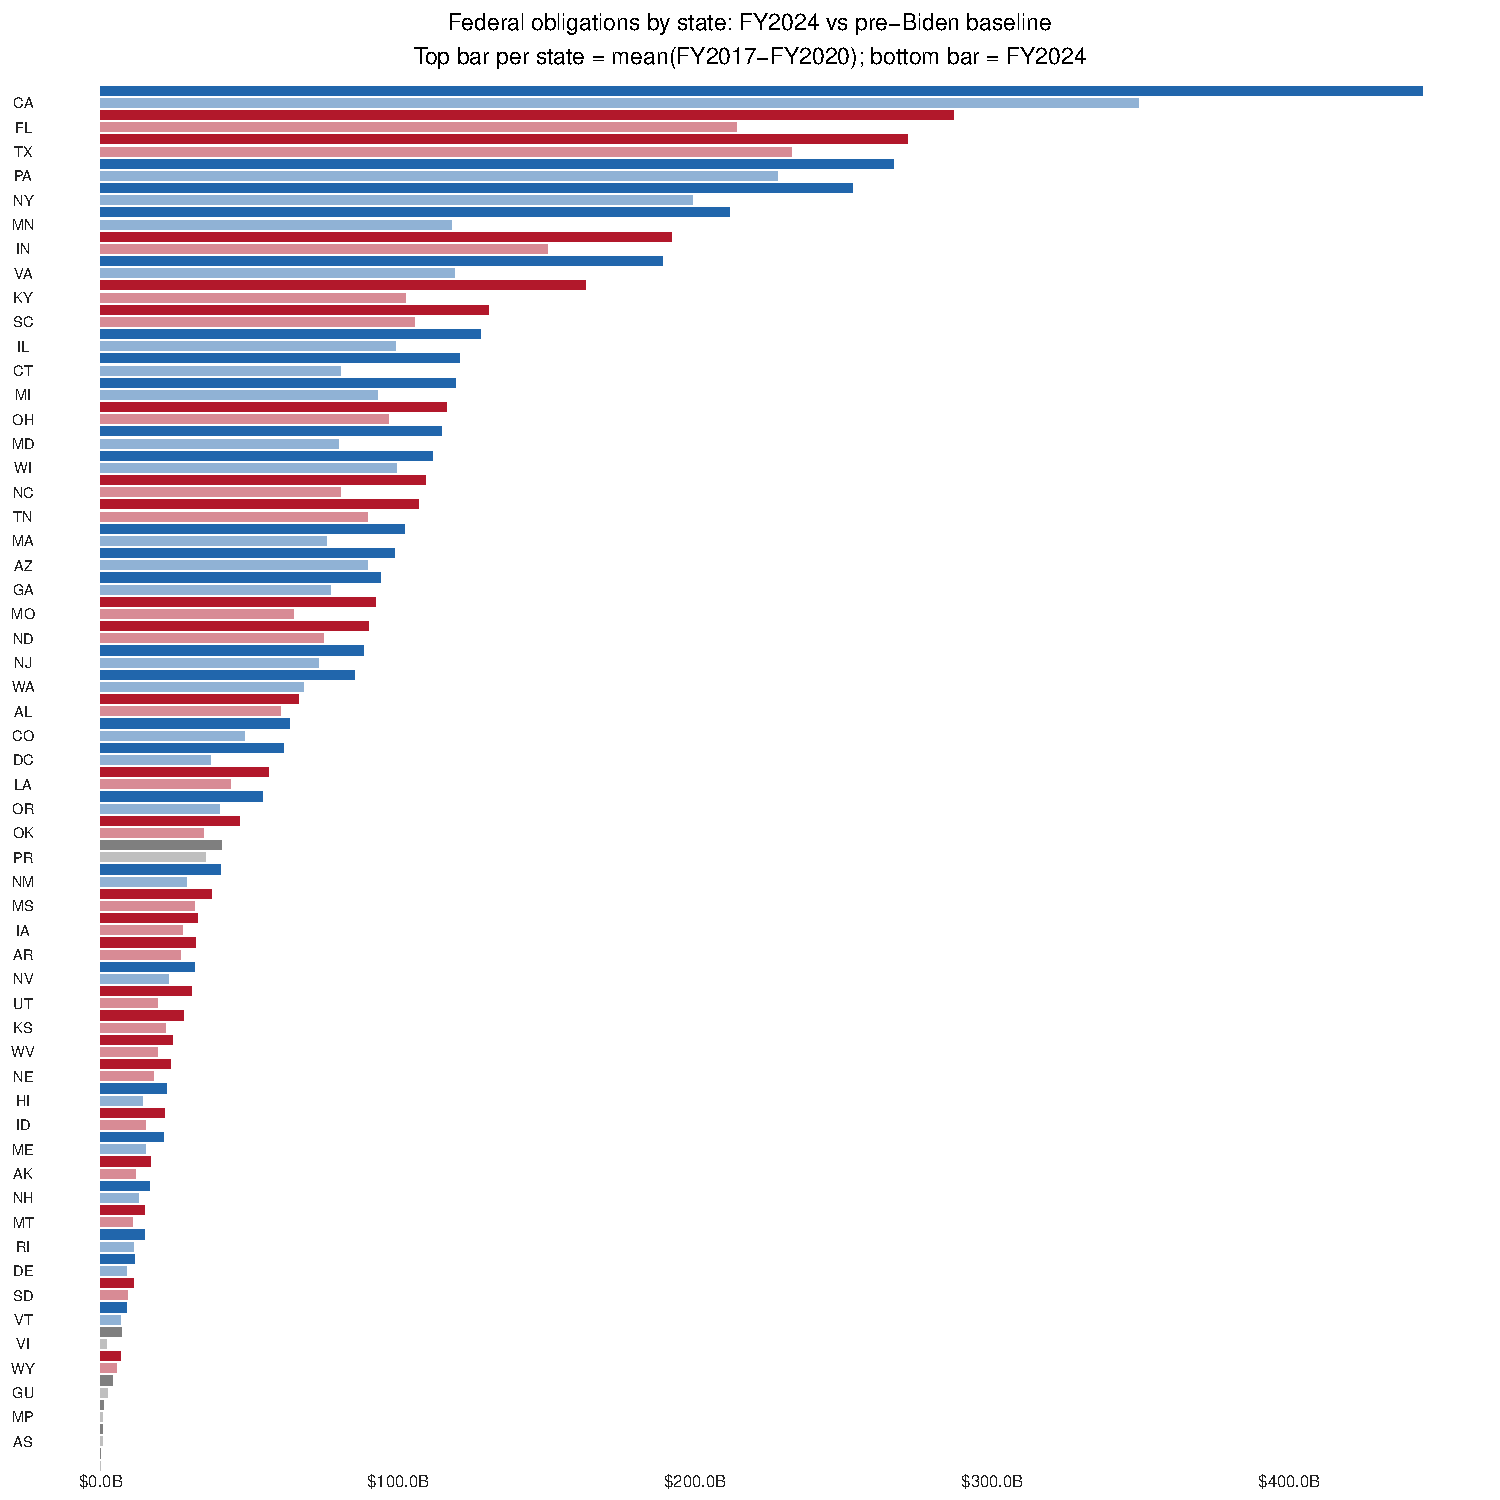
\includegraphics[keepaspectratio]{spending_elections_2020_2024_analysis_patched_files/figure-latex/bar-total-compare-1.pdf}}

\subsubsection{Key Observations}\label{key-observations}

\begin{enumerate}
\def\labelenumi{\arabic{enumi}.}
\item
  \textbf{Why data beyond the IIJA snapshot:} The IIJA spreadsheet is a
  program‑specific funding snapshot, but the research question requires
  \textbf{total federal obligations} across all programs. The
  USAspending API provides full‑scope spending needed to compare eras
  and align with election outcomes.
\item
  \textbf{Comparable time windows:} Using FY2017--FY2020 vs FY2024
  creates a stable baseline instead of a single year or a single
  program, making changes more interpretable.
\end{enumerate}

\subsection{FY2024 Obligations Per Capita by
State}\label{fy2024-obligations-per-capita-by-state}

\begin{Shaded}
\begin{Highlighting}[]
\CommentTok{\# Ensure consistent series ordering within each state: Pre above FY2024}
\NormalTok{pre\_lab }\OtherTok{\textless{}{-}} \StringTok{"Pre (FY17–FY20 avg)"}
\NormalTok{fy24\_lab }\OtherTok{\textless{}{-}} \StringTok{"FY2024"}

\CommentTok{\# Order states by the maximum of the two series for readability}
\NormalTok{state\_order\_pc }\OtherTok{\textless{}{-}}\NormalTok{ bars\_pc }\SpecialCharTok{|\textgreater{}}
  \FunctionTok{group\_by}\NormalTok{(state) }\SpecialCharTok{|\textgreater{}}
  \FunctionTok{summarize}\NormalTok{(}\AttributeTok{max\_val =} \FunctionTok{max}\NormalTok{(value, }\AttributeTok{na.rm =} \ConstantTok{TRUE}\NormalTok{), }\AttributeTok{.groups =} \StringTok{"drop"}\NormalTok{) }\SpecialCharTok{|\textgreater{}}
  \FunctionTok{arrange}\NormalTok{(max\_val) }\SpecialCharTok{|\textgreater{}}
  \FunctionTok{pull}\NormalTok{(state)}

\CommentTok{\# Force y{-}axis levels: for each state, Pre then FY2024}
\NormalTok{y\_levels\_pc }\OtherTok{\textless{}{-}} \FunctionTok{c}\NormalTok{(}\FunctionTok{rbind}\NormalTok{(}
  \FunctionTok{paste0}\NormalTok{(state\_order\_pc, }\StringTok{"  "}\NormalTok{, pre\_lab),}
  \FunctionTok{paste0}\NormalTok{(state\_order\_pc, }\StringTok{"  "}\NormalTok{, fy24\_lab)}
\NormalTok{))}

\NormalTok{bars\_pc\_plot }\OtherTok{\textless{}{-}}\NormalTok{ bars\_pc }\SpecialCharTok{|\textgreater{}}
  \FunctionTok{mutate}\NormalTok{(}
    \AttributeTok{series =} \FunctionTok{factor}\NormalTok{(series, }\AttributeTok{levels =} \FunctionTok{c}\NormalTok{(pre\_lab, fy24\_lab)),}
    \AttributeTok{alpha\_series =} \FunctionTok{if\_else}\NormalTok{(series }\SpecialCharTok{==}\NormalTok{ pre\_lab, }\FloatTok{0.5}\NormalTok{, }\FloatTok{1.0}\NormalTok{),}
    \AttributeTok{state\_series =} \FunctionTok{paste0}\NormalTok{(state, }\StringTok{"  "}\NormalTok{, }\FunctionTok{as.character}\NormalTok{(series)),}
    \AttributeTok{state\_series =} \FunctionTok{factor}\NormalTok{(state\_series, }\AttributeTok{levels =}\NormalTok{ y\_levels\_pc)}
\NormalTok{  )}

\FunctionTok{ggplot}\NormalTok{(bars\_pc\_plot, }\FunctionTok{aes}\NormalTok{(}\AttributeTok{x =}\NormalTok{ value, }\AttributeTok{y =}\NormalTok{ state\_series, }\AttributeTok{fill =}\NormalTok{ winner\_2020, }\AttributeTok{alpha =}\NormalTok{ alpha\_series)) }\SpecialCharTok{+}
  \FunctionTok{geom\_col}\NormalTok{(}\AttributeTok{width =} \FloatTok{0.75}\NormalTok{) }\SpecialCharTok{+}
  \FunctionTok{scale\_party\_fill}\NormalTok{() }\SpecialCharTok{+}
  \FunctionTok{scale\_alpha\_identity}\NormalTok{(}\AttributeTok{guide =} \StringTok{"none"}\NormalTok{) }\SpecialCharTok{+}
  \FunctionTok{scale\_y\_discrete}\NormalTok{(}\AttributeTok{labels =} \ControlFlowTok{function}\NormalTok{(x) \{}
\NormalTok{    st }\OtherTok{\textless{}{-}} \FunctionTok{sub}\NormalTok{(}\StringTok{"  .*"}\NormalTok{, }\StringTok{""}\NormalTok{, x)}
    \FunctionTok{ifelse}\NormalTok{(}\FunctionTok{duplicated}\NormalTok{(st), }\StringTok{""}\NormalTok{, st)}
\NormalTok{  \}) }\SpecialCharTok{+}
  \FunctionTok{scale\_x\_continuous}\NormalTok{(}\AttributeTok{labels =}\NormalTok{ label\_dollars1) }\SpecialCharTok{+}
  \FunctionTok{labs}\NormalTok{(}
    \AttributeTok{title =} \StringTok{"Federal obligations per capita by state: FY2024 vs pre{-}Biden baseline"}\NormalTok{,}
    \AttributeTok{subtitle =} \StringTok{"Top bar per state = mean(FY2017{-}FY2020); bottom bar = FY2024"}\NormalTok{,}
    \AttributeTok{x =} \StringTok{"Obligations per capita ($)"}\NormalTok{,}
    \AttributeTok{y =} \ConstantTok{NULL}
\NormalTok{  ) }\SpecialCharTok{+}
  \FunctionTok{theme\_low\_ink}\NormalTok{() }\SpecialCharTok{+}
  \FunctionTok{theme}\NormalTok{(}
    \AttributeTok{panel.grid.major =} \FunctionTok{element\_blank}\NormalTok{(),}
    \AttributeTok{panel.grid.minor =} \FunctionTok{element\_blank}\NormalTok{(),}
    \AttributeTok{axis.line =} \FunctionTok{element\_blank}\NormalTok{(),}
    \AttributeTok{axis.ticks =} \FunctionTok{element\_blank}\NormalTok{(),}
    \AttributeTok{axis.text.y =} \FunctionTok{element\_text}\NormalTok{(}\AttributeTok{size =} \DecValTok{7}\NormalTok{)}
\NormalTok{  )}
\end{Highlighting}
\end{Shaded}

\pandocbounded{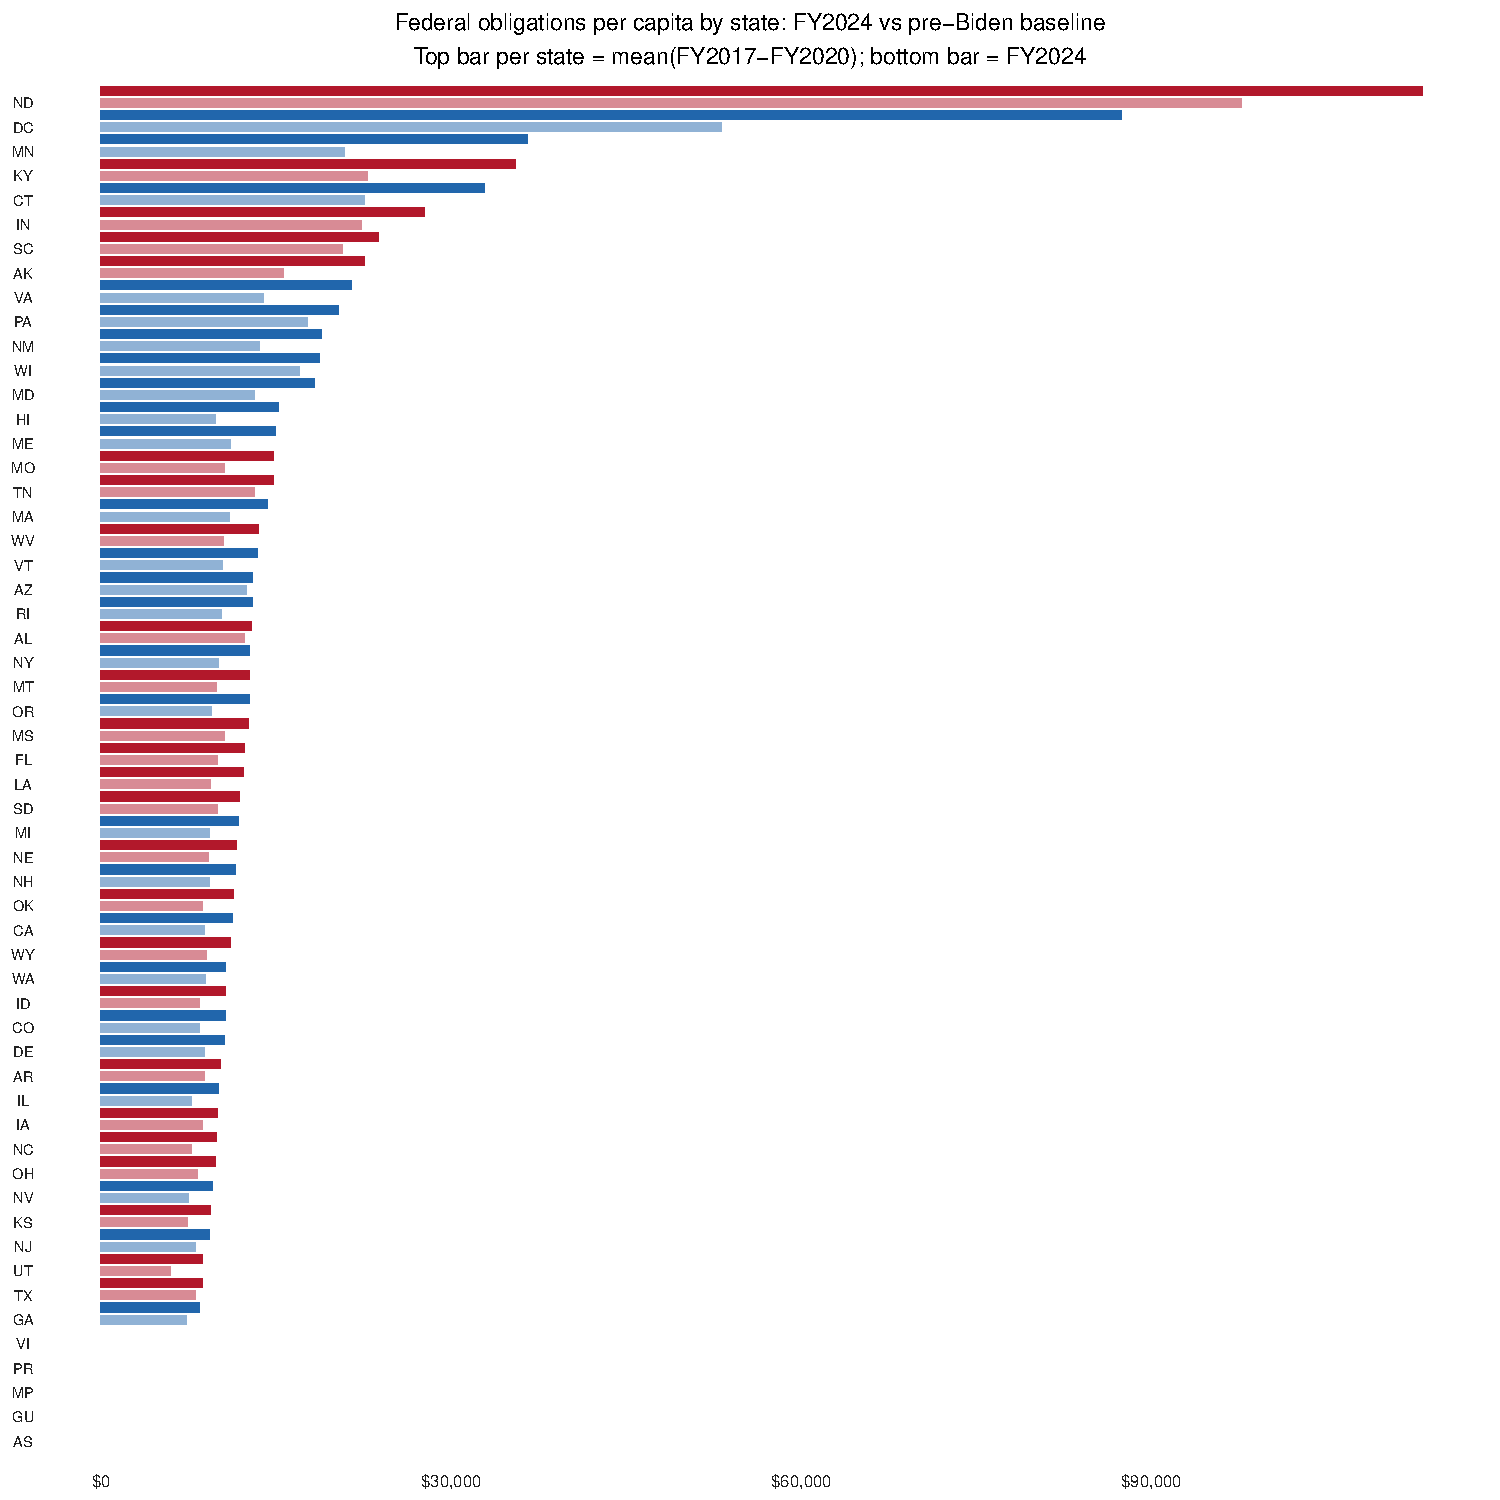
\includegraphics[keepaspectratio]{spending_elections_2020_2024_analysis_patched_files/figure-latex/bar-pc-compare-1.pdf}}

\subsubsection{Key Observations}\label{key-observations-1}

\begin{enumerate}
\def\labelenumi{\arabic{enumi}.}
\item
  \textbf{Why per‑capita is clearer:} Per‑capita spending controls for
  population size, revealing states that look small in total dollars but
  large \textbf{per resident}.
\item
  \textbf{Per‑capita pitfalls:} Very small population states and DC can
  show extreme values because the denominator is small. These outliers
  are real but can \textbf{exaggerate swings}, so they should be read
  alongside totals.
\end{enumerate}

\section{IIJA Funding Snapshot (March
2023)}\label{iija-funding-snapshot-march-2023}

This chart uses the \textbf{IIJA funding snapshot (as of March 2023)} to
provide a program-specific view alongside the all-program USAspending
totals. The snapshot is not a substitute for total obligations, but it
offers a focused look at infrastructure-specific allocations, which is
why other datasets are used for the broader spending and election
comparisons.

\begin{Shaded}
\begin{Highlighting}[]
\ControlFlowTok{if}\NormalTok{ (}\SpecialCharTok{!}\FunctionTok{is.null}\NormalTok{(iija) }\SpecialCharTok{\&\&} \FunctionTok{nrow}\NormalTok{(iija) }\SpecialCharTok{\textgreater{}} \DecValTok{0} \SpecialCharTok{\&\&} \FunctionTok{exists}\NormalTok{(}\StringTok{"pop"}\NormalTok{)) \{}

\NormalTok{  iija\_plot }\OtherTok{\textless{}{-}}\NormalTok{ iija }\SpecialCharTok{|\textgreater{}}
    \FunctionTok{filter}\NormalTok{(state }\SpecialCharTok{\%in\%} \FunctionTok{c}\NormalTok{(state.abb, }\StringTok{"DC"}\NormalTok{)) }\SpecialCharTok{|\textgreater{}}
    \FunctionTok{left\_join}\NormalTok{(pop }\SpecialCharTok{|\textgreater{}}
                \FunctionTok{filter}\NormalTok{(fiscal\_year }\SpecialCharTok{==} \DecValTok{2023}\NormalTok{) }\SpecialCharTok{|\textgreater{}}
                \FunctionTok{select}\NormalTok{(state, }\AttributeTok{pop\_2023 =}\NormalTok{ pop),}
              \AttributeTok{by =} \StringTok{"state"}\NormalTok{) }\SpecialCharTok{|\textgreater{}}
    \FunctionTok{mutate}\NormalTok{(}
      \AttributeTok{iija\_total =}\NormalTok{ iija\_total\_bil }\SpecialCharTok{*} \FloatTok{1e9}\NormalTok{,}
      \AttributeTok{iija\_pc =}\NormalTok{ iija\_total }\SpecialCharTok{/}\NormalTok{ pop\_2023}
\NormalTok{    ) }\SpecialCharTok{|\textgreater{}}
    \FunctionTok{left\_join}\NormalTok{(pres2020 }\SpecialCharTok{|\textgreater{}} \FunctionTok{select}\NormalTok{(state, winner\_2020), }\AttributeTok{by =} \StringTok{"state"}\NormalTok{) }\SpecialCharTok{|\textgreater{}}
    \FunctionTok{arrange}\NormalTok{(iija\_pc) }\SpecialCharTok{|\textgreater{}}
    \FunctionTok{mutate}\NormalTok{(}\AttributeTok{state =} \FunctionTok{factor}\NormalTok{(state, }\AttributeTok{levels =}\NormalTok{ state))}

  \FunctionTok{ggplot}\NormalTok{(iija\_plot, }\FunctionTok{aes}\NormalTok{(}\AttributeTok{x =}\NormalTok{ iija\_pc, }\AttributeTok{y =}\NormalTok{ state, }\AttributeTok{fill =}\NormalTok{ winner\_2020)) }\SpecialCharTok{+}
    \FunctionTok{geom\_col}\NormalTok{(}\AttributeTok{width =} \FloatTok{0.75}\NormalTok{) }\SpecialCharTok{+}
    \FunctionTok{scale\_party\_fill}\NormalTok{(}\AttributeTok{guide =} \StringTok{"none"}\NormalTok{) }\SpecialCharTok{+}
    \FunctionTok{scale\_x\_continuous}\NormalTok{(}\AttributeTok{labels =}\NormalTok{ label\_dollars1) }\SpecialCharTok{+}
    \FunctionTok{labs}\NormalTok{(}
      \AttributeTok{title =} \StringTok{"IIJA funding per capita by state (March 2023 snapshot)"}\NormalTok{,}
      \AttributeTok{subtitle =} \StringTok{"Program{-}specific snapshot; per{-}capita uses 2023 population"}\NormalTok{,}
      \AttributeTok{x =} \StringTok{"IIJA funding per capita ($)"}\NormalTok{,}
      \AttributeTok{y =} \ConstantTok{NULL}
\NormalTok{    ) }\SpecialCharTok{+}
    \FunctionTok{theme\_low\_ink}\NormalTok{() }\SpecialCharTok{+}
    \FunctionTok{theme}\NormalTok{(}
      \AttributeTok{panel.grid.major =} \FunctionTok{element\_blank}\NormalTok{(),}
      \AttributeTok{panel.grid.minor =} \FunctionTok{element\_blank}\NormalTok{(),}
      \AttributeTok{axis.line =} \FunctionTok{element\_blank}\NormalTok{(),}
      \AttributeTok{axis.ticks =} \FunctionTok{element\_blank}\NormalTok{(),}
      \AttributeTok{axis.text.y =} \FunctionTok{element\_text}\NormalTok{(}\AttributeTok{size =} \DecValTok{7}\NormalTok{)}
\NormalTok{    )}
\NormalTok{\} }\ControlFlowTok{else}\NormalTok{ \{}
  \FunctionTok{message}\NormalTok{(}\StringTok{"IIJA snapshot not available. Ensure the Excel file is present."}\NormalTok{)}
\NormalTok{\}}
\end{Highlighting}
\end{Shaded}

\pandocbounded{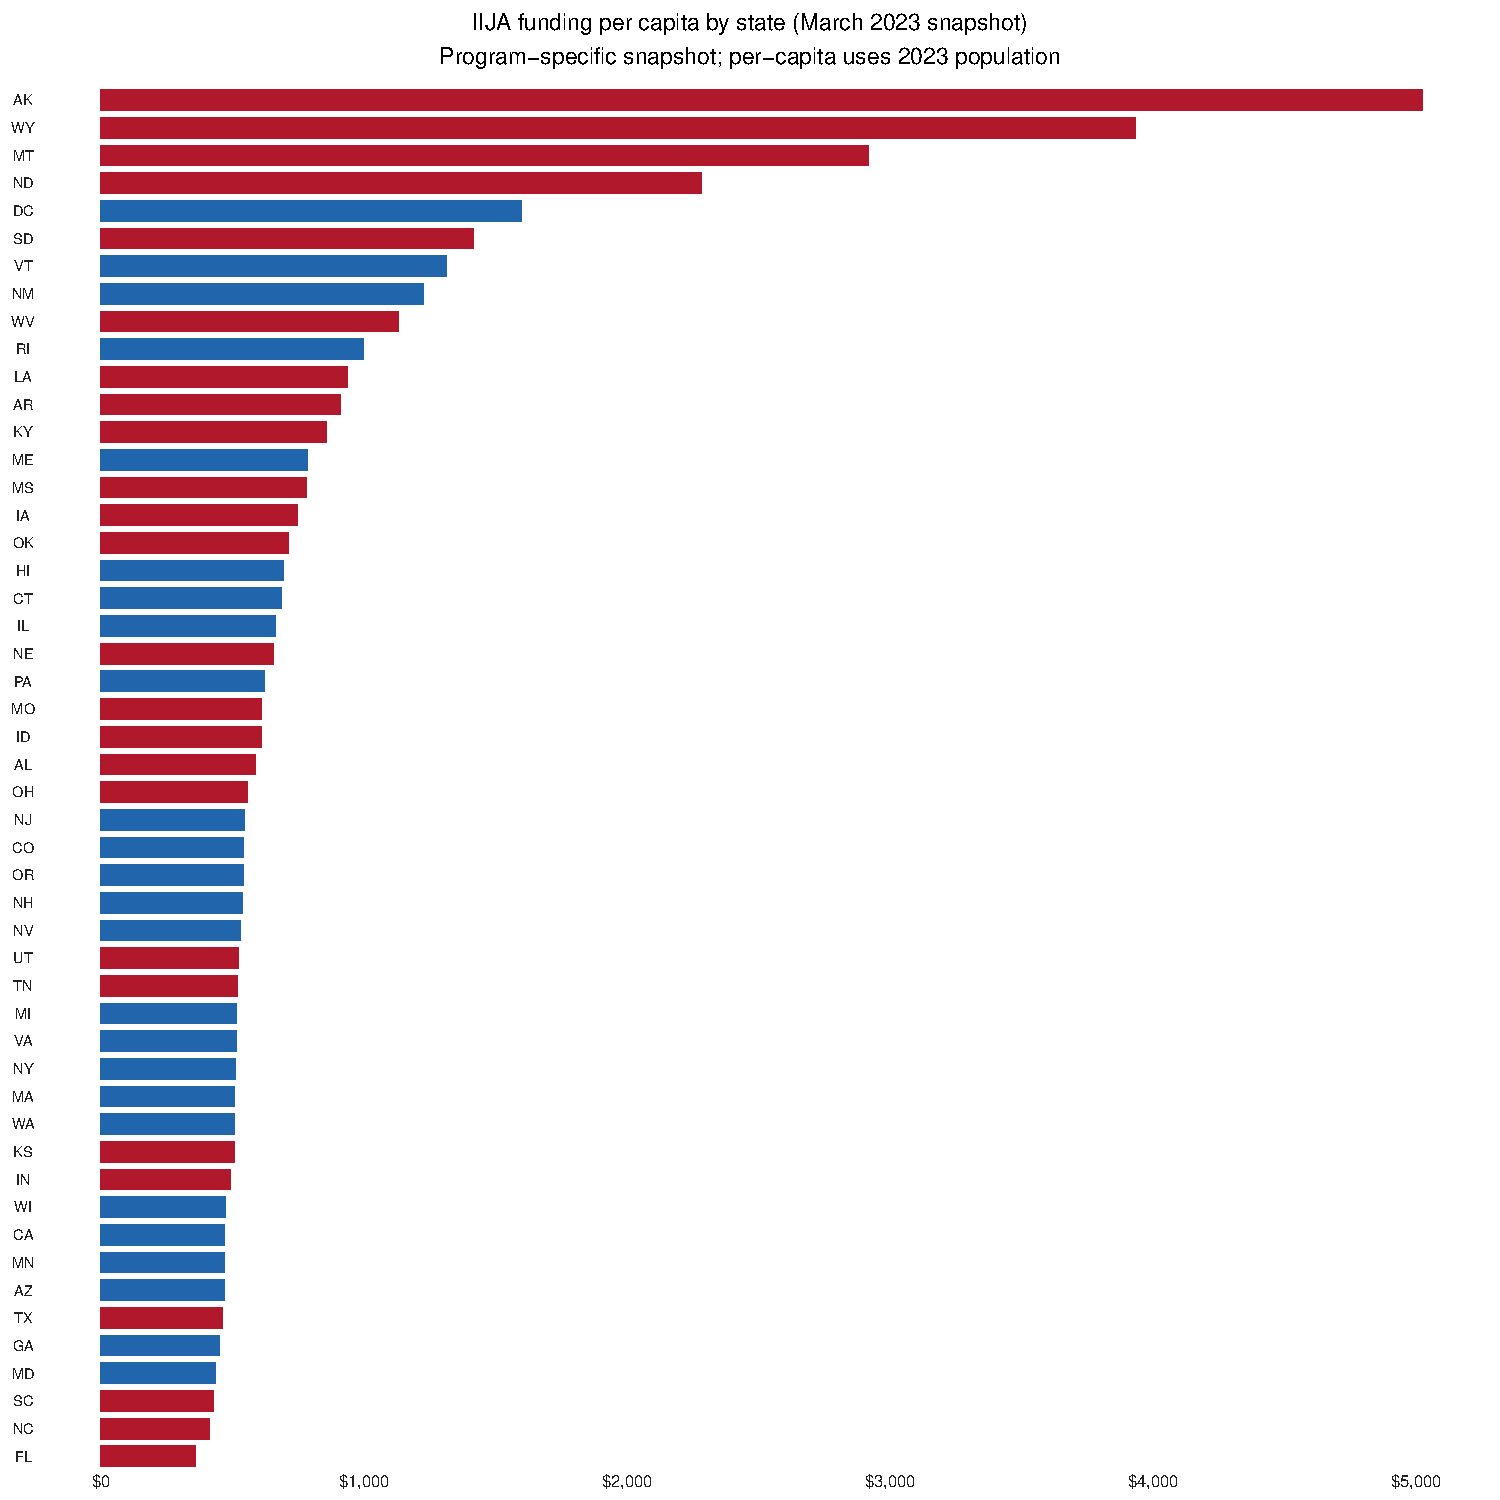
\includegraphics[keepaspectratio]{spending_elections_2020_2024_analysis_patched_files/figure-latex/iija-snapshot-1.pdf}}

\subsubsection{Key Observations}\label{key-observations-2}

\begin{enumerate}
\def\labelenumi{\arabic{enumi}.}
\item
  \textbf{Program-specific contrast:} This IIJA snapshot shows
  infrastructure allocations only, which can diverge from overall
  federal obligations shown in the earlier charts.
\item
  \textbf{Per-capita framing:} Using 2023 population normalizes for
  state size, highlighting smaller states with higher infrastructure
  dollars per resident.
\end{enumerate}

\section{2024 Election Results}\label{election-results}

\begin{Shaded}
\begin{Highlighting}[]
\NormalTok{states\_2024 }\OtherTok{\textless{}{-}} \FunctionTok{read\_csv}\NormalTok{(}\StringTok{"https://michaelminn.net/tutorials/data/2024{-}electoral{-}states.csv"}\NormalTok{) }\SpecialCharTok{|\textgreater{}} \FunctionTok{clean\_names}\NormalTok{()}
\NormalTok{districts\_2024 }\OtherTok{\textless{}{-}} \FunctionTok{read\_csv}\NormalTok{(}\StringTok{"https://michaelminn.net/tutorials/data/2024{-}electoral{-}districts.csv"}\NormalTok{) }\SpecialCharTok{|\textgreater{}} \FunctionTok{clean\_names}\NormalTok{()}

\NormalTok{pres\_2024 }\OtherTok{\textless{}{-}}\NormalTok{ states\_2024 }\SpecialCharTok{|\textgreater{}}
  \FunctionTok{transmute}\NormalTok{(}
    \AttributeTok{state =}\NormalTok{ st,}
    \AttributeTok{pres\_margin\_dem =}\NormalTok{ (votes\_dem\_2024 }\SpecialCharTok{{-}}\NormalTok{ votes\_gop\_2024) }\SpecialCharTok{/}
\NormalTok{      (votes\_dem\_2024 }\SpecialCharTok{+}\NormalTok{ votes\_gop\_2024)}
\NormalTok{  )}

\NormalTok{house\_2024 }\OtherTok{\textless{}{-}}\NormalTok{ districts\_2024 }\SpecialCharTok{|\textgreater{}}
  \FunctionTok{group\_by}\NormalTok{(st) }\SpecialCharTok{|\textgreater{}}
  \FunctionTok{summarize}\NormalTok{(}
    \AttributeTok{house\_margin\_dem =}
\NormalTok{      (}\FunctionTok{sum}\NormalTok{(votes\_dem\_2024) }\SpecialCharTok{{-}} \FunctionTok{sum}\NormalTok{(votes\_gop\_2024)) }\SpecialCharTok{/}
\NormalTok{      (}\FunctionTok{sum}\NormalTok{(votes\_dem\_2024) }\SpecialCharTok{+} \FunctionTok{sum}\NormalTok{(votes\_gop\_2024)),}
    \AttributeTok{.groups =} \StringTok{"drop"}
\NormalTok{  ) }\SpecialCharTok{|\textgreater{}}
  \FunctionTok{rename}\NormalTok{(}\AttributeTok{state =}\NormalTok{ st)}

\NormalTok{elections\_2024 }\OtherTok{\textless{}{-}} \FunctionTok{left\_join}\NormalTok{(pres\_2024, house\_2024, }\AttributeTok{by =} \StringTok{"state"}\NormalTok{)}
\end{Highlighting}
\end{Shaded}

\section{Merge Spending and
Elections}\label{merge-spending-and-elections}

\begin{Shaded}
\begin{Highlighting}[]
\NormalTok{analysis }\OtherTok{\textless{}{-}}\NormalTok{ delta\_12\_1 }\SpecialCharTok{|\textgreater{}}
  \FunctionTok{select}\NormalTok{(state, delta\_biden\_vs\_pre\_pc) }\SpecialCharTok{|\textgreater{}}
  \FunctionTok{left\_join}\NormalTok{(elections\_2024, }\AttributeTok{by =} \StringTok{"state"}\NormalTok{)}
\end{Highlighting}
\end{Shaded}

\section{Results}\label{results}

\subsection{Spending Change vs 2024 Presidential
Margin}\label{spending-change-vs-2024-presidential-margin}

\begin{Shaded}
\begin{Highlighting}[]
\NormalTok{pres\_plot\_data }\OtherTok{\textless{}{-}}\NormalTok{ analysis }\SpecialCharTok{|\textgreater{}}
  \FunctionTok{filter}\NormalTok{(}\SpecialCharTok{!}\FunctionTok{is.na}\NormalTok{(pres\_margin\_dem))}

\NormalTok{pres\_lm }\OtherTok{\textless{}{-}} \FunctionTok{lm}\NormalTok{(pres\_margin\_dem }\SpecialCharTok{\textasciitilde{}}\NormalTok{ delta\_biden\_vs\_pre\_pc, }\AttributeTok{data =}\NormalTok{ pres\_plot\_data)}
\NormalTok{pres\_r2 }\OtherTok{\textless{}{-}} \FunctionTok{summary}\NormalTok{(pres\_lm)}\SpecialCharTok{$}\NormalTok{r.squared}
\NormalTok{pres\_p }\OtherTok{\textless{}{-}} \FunctionTok{summary}\NormalTok{(pres\_lm)}\SpecialCharTok{$}\NormalTok{coefficients[}\DecValTok{2}\NormalTok{, }\DecValTok{4}\NormalTok{]}

\NormalTok{pres\_label }\OtherTok{\textless{}{-}} \FunctionTok{sprintf}\NormalTok{(}\StringTok{"R2 = \%.3f}\SpecialCharTok{\textbackslash{}n}\StringTok{p = \%.3g"}\NormalTok{, pres\_r2, pres\_p)}

\FunctionTok{ggplot}\NormalTok{(pres\_plot\_data, }\FunctionTok{aes}\NormalTok{(delta\_biden\_vs\_pre\_pc, pres\_margin\_dem)) }\SpecialCharTok{+}
  \FunctionTok{geom\_hline}\NormalTok{(}\AttributeTok{yintercept =} \DecValTok{0}\NormalTok{, }\AttributeTok{linewidth =} \FloatTok{0.25}\NormalTok{) }\SpecialCharTok{+}
  \FunctionTok{geom\_vline}\NormalTok{(}\AttributeTok{xintercept =} \DecValTok{0}\NormalTok{, }\AttributeTok{linewidth =} \FloatTok{0.25}\NormalTok{) }\SpecialCharTok{+}
  \FunctionTok{geom\_point}\NormalTok{() }\SpecialCharTok{+}
  \FunctionTok{geom\_smooth}\NormalTok{(}\AttributeTok{method =} \StringTok{"lm"}\NormalTok{, }\AttributeTok{se =} \ConstantTok{FALSE}\NormalTok{) }\SpecialCharTok{+}
  \FunctionTok{annotate}\NormalTok{(}
    \StringTok{"label"}\NormalTok{,}
    \AttributeTok{x =} \ConstantTok{Inf}\NormalTok{, }\AttributeTok{y =} \ConstantTok{Inf}\NormalTok{,}
    \AttributeTok{label =}\NormalTok{ pres\_label,}
    \AttributeTok{hjust =} \FloatTok{1.1}\NormalTok{, }\AttributeTok{vjust =} \FloatTok{1.1}\NormalTok{,}
    \AttributeTok{size =} \DecValTok{4}\NormalTok{,}
    \AttributeTok{label.size =} \FloatTok{0.25}\NormalTok{,}
    \AttributeTok{fill =} \StringTok{"white"}\NormalTok{,}
    \AttributeTok{color =} \StringTok{"black"}
\NormalTok{  ) }\SpecialCharTok{+}
  \FunctionTok{scale\_x\_continuous}\NormalTok{(}\AttributeTok{labels =}\NormalTok{ dollar) }\SpecialCharTok{+}
  \FunctionTok{scale\_y\_continuous}\NormalTok{(}\AttributeTok{labels =}\NormalTok{ percent) }\SpecialCharTok{+}
  \FunctionTok{labs}\NormalTok{(}
    \AttributeTok{title =} \StringTok{"Change in Federal Spending (Biden Era vs Pre{-}Biden) vs 2024 Presidential Margin"}\NormalTok{,}
    \AttributeTok{x =} \StringTok{"Δ Federal Obligations per Capita (mean FY2021–FY2024 − mean FY2017–FY2020)"}\NormalTok{,}
    \AttributeTok{y =} \StringTok{"2024 Presidential Margin (Dem − GOP)"}
\NormalTok{  )}
\end{Highlighting}
\end{Shaded}

\pandocbounded{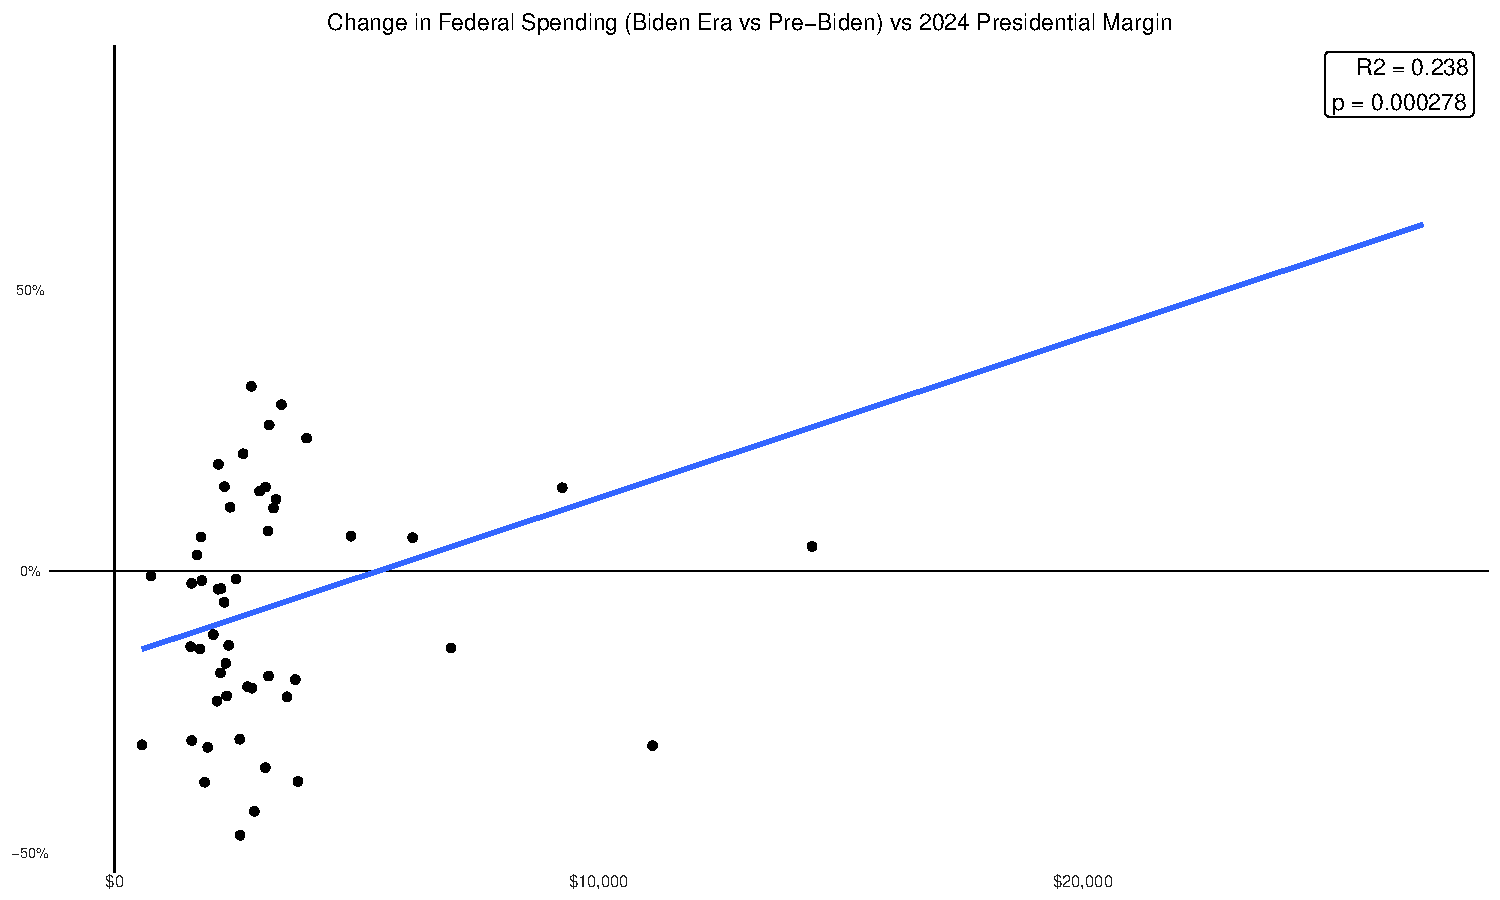
\includegraphics[keepaspectratio]{spending_elections_2020_2024_analysis_patched_files/figure-latex/plot-pres-1.pdf}}

\subsection{Key Observations}\label{key-observations-3}

\textbf{What This Chart Shows:}

This scatter plot examines whether average federal spending per capita
in the Biden era (FY2021--FY2024) versus the pre-Biden baseline
(FY2017--FY2020) correlates with how states voted in the 2024
presidential election. Each point represents one state (or DC), with:

\begin{itemize}
\tightlist
\item
  X-axis: Change in federal obligations per capita (positive = higher
  Biden-era average than pre-Biden)
\item
  Y-axis: 2024 Presidential margin (positive = Democratic win; negative
  = Republican win)
\item
  Fitted line: Linear regression showing the overall trend across all
  jurisdictions
\end{itemize}

\subsubsection{Analytical Findings:}\label{analytical-findings}

\begin{enumerate}
\def\labelenumi{\arabic{enumi}.}
\item
  \textbf{Moderate Positive Association:} The fitted line is upward
  sloping, with a correlation of about \textbf{0.49} and an \textbf{R2
  \textasciitilde{} 0.24}. States with larger per-capita spending
  increases tended to have more Democratic 2024 presidential margins,
  though the relationship is far from deterministic.
\item
  \textbf{All States Show Positive Spending Change:} Because this
  compares two multi-year averages, every state has a positive delta.
  That means all points fall in the \textbf{positive-spending} half,
  split between \textbf{Dem margins (20 states)} and \textbf{GOP margins
  (31 states)}. The partisan split underscores that spending increases
  did not uniformly translate into electoral support.
\item
  \textbf{Notable Outliers:} Several states sit far from the trend line,
  suggesting other forces dominate:
\end{enumerate}

\begin{itemize}
\tightlist
\item
  \textbf{KY}: large spending increase but strong GOP margin
\item
  \textbf{VT}: moderate spending increase paired with strong Democratic
  margin
\item
  \textbf{WY}, \textbf{WV}, \textbf{MD}: sizable residuals in opposite
  directions
\end{itemize}

\begin{enumerate}
\def\labelenumi{\arabic{enumi}.}
\setcounter{enumi}{3}
\tightlist
\item
  \textbf{Correlation, Not Causation:} Even with a measurable
  association, this remains observational. Spending levels, state
  economies, and political alignment interact in ways this bivariate
  plot cannot disentangle.
\end{enumerate}

\subsection{Spending Change vs 2024 House
Margin}\label{spending-change-vs-2024-house-margin}

\begin{Shaded}
\begin{Highlighting}[]
\NormalTok{house\_plot\_data }\OtherTok{\textless{}{-}}\NormalTok{ analysis }\SpecialCharTok{|\textgreater{}}
  \FunctionTok{filter}\NormalTok{(}\SpecialCharTok{!}\FunctionTok{is.na}\NormalTok{(house\_margin\_dem))}

\NormalTok{house\_lm }\OtherTok{\textless{}{-}} \FunctionTok{lm}\NormalTok{(house\_margin\_dem }\SpecialCharTok{\textasciitilde{}}\NormalTok{ delta\_biden\_vs\_pre\_pc, }\AttributeTok{data =}\NormalTok{ house\_plot\_data)}
\NormalTok{house\_r2 }\OtherTok{\textless{}{-}} \FunctionTok{summary}\NormalTok{(house\_lm)}\SpecialCharTok{$}\NormalTok{r.squared}
\NormalTok{house\_p }\OtherTok{\textless{}{-}} \FunctionTok{summary}\NormalTok{(house\_lm)}\SpecialCharTok{$}\NormalTok{coefficients[}\DecValTok{2}\NormalTok{, }\DecValTok{4}\NormalTok{]}

\NormalTok{house\_label }\OtherTok{\textless{}{-}} \FunctionTok{sprintf}\NormalTok{(}\StringTok{"R2 = \%.3f}\SpecialCharTok{\textbackslash{}n}\StringTok{p = \%.3g"}\NormalTok{, house\_r2, house\_p)}

\FunctionTok{ggplot}\NormalTok{(house\_plot\_data, }\FunctionTok{aes}\NormalTok{(delta\_biden\_vs\_pre\_pc, house\_margin\_dem)) }\SpecialCharTok{+}
  \FunctionTok{geom\_hline}\NormalTok{(}\AttributeTok{yintercept =} \DecValTok{0}\NormalTok{, }\AttributeTok{linewidth =} \FloatTok{0.25}\NormalTok{) }\SpecialCharTok{+}
  \FunctionTok{geom\_vline}\NormalTok{(}\AttributeTok{xintercept =} \DecValTok{0}\NormalTok{, }\AttributeTok{linewidth =} \FloatTok{0.25}\NormalTok{) }\SpecialCharTok{+}
  \FunctionTok{geom\_point}\NormalTok{() }\SpecialCharTok{+}
  \FunctionTok{geom\_smooth}\NormalTok{(}\AttributeTok{method =} \StringTok{"lm"}\NormalTok{, }\AttributeTok{se =} \ConstantTok{FALSE}\NormalTok{) }\SpecialCharTok{+}
  \FunctionTok{annotate}\NormalTok{(}
    \StringTok{"label"}\NormalTok{,}
    \AttributeTok{x =} \ConstantTok{Inf}\NormalTok{, }\AttributeTok{y =} \ConstantTok{Inf}\NormalTok{,}
    \AttributeTok{label =}\NormalTok{ house\_label,}
    \AttributeTok{hjust =} \FloatTok{1.1}\NormalTok{, }\AttributeTok{vjust =} \FloatTok{1.1}\NormalTok{,}
    \AttributeTok{size =} \DecValTok{4}\NormalTok{,}
    \AttributeTok{label.size =} \FloatTok{0.25}\NormalTok{,}
    \AttributeTok{fill =} \StringTok{"white"}\NormalTok{,}
    \AttributeTok{color =} \StringTok{"black"}
\NormalTok{  ) }\SpecialCharTok{+}
  \FunctionTok{scale\_x\_continuous}\NormalTok{(}\AttributeTok{labels =}\NormalTok{ dollar) }\SpecialCharTok{+}
  \FunctionTok{scale\_y\_continuous}\NormalTok{(}\AttributeTok{labels =}\NormalTok{ percent) }\SpecialCharTok{+}
  \FunctionTok{labs}\NormalTok{(}
    \AttributeTok{title =} \StringTok{"Change in Federal Spending (Biden Era vs Pre{-}Biden) vs 2024 House Margin"}\NormalTok{,}
    \AttributeTok{x =} \StringTok{"Δ Federal Obligations per Capita (mean FY2021–FY2024 − mean FY2017–FY2020)"}\NormalTok{,}
    \AttributeTok{y =} \StringTok{"2024 House Margin (Dem − GOP)"}
\NormalTok{  )}
\end{Highlighting}
\end{Shaded}

\pandocbounded{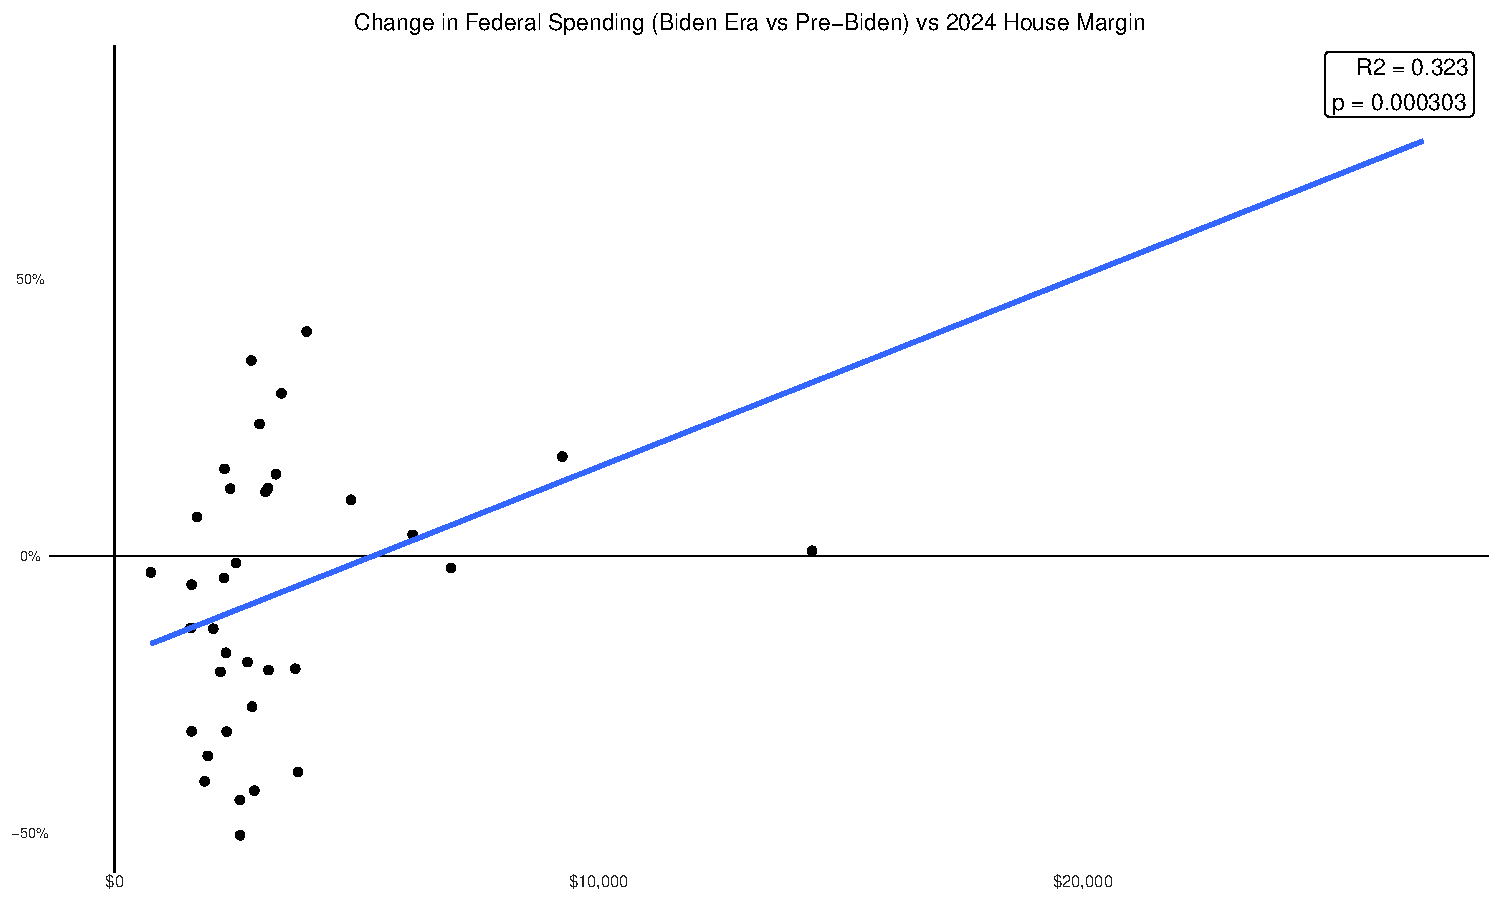
\includegraphics[keepaspectratio]{spending_elections_2020_2024_analysis_patched_files/figure-latex/plot-house-1.pdf}}

\subsection{Key Observations}\label{key-observations-4}

\textbf{What This Chart Shows:}

This scatter plot tests whether federal spending changes correlate with
aggregate House election outcomes at the state level. The analysis uses:

\begin{itemize}
\tightlist
\item
  X-axis: Change in federal obligations per capita (FY2024 − FY2020)
\item
  Y-axis: State-level House margin (total Democratic votes − total
  Republican votes across all districts)
\item
  Fitted line: Linear regression trend
\end{itemize}

\subsubsection{Analytical Findings:}\label{analytical-findings-1}

\begin{enumerate}
\def\labelenumi{\arabic{enumi}.}
\item
  \textbf{Moderate Positive Association:} The House margin relationship
  is somewhat stronger, with a correlation of about \textbf{0.57} and
  \textbf{R2 \textasciitilde{} 0.32}. States with larger spending
  increases generally show more Democratic House margins, though there
  is still substantial dispersion.
\item
  \textbf{District Aggregation Still Blurs Signal:} House results are
  the sum of many district contests. A state's aggregate margin can mask
  district‑level swings that are unrelated to statewide spending
  changes.
\item
  \textbf{Outliers Highlight Local Dynamics:} States with large
  residuals include \textbf{HI}, \textbf{VT}, \textbf{WY}, \textbf{MD},
  and \textbf{SD}, indicating that local political factors can overwhelm
  any spending-related pattern.
\item
  \textbf{Correlation, Not Causation:} As with the presidential plot,
  this is an observational association. The chart does not establish
  whether spending affects votes or whether both reflect deeper
  structural factors.
\end{enumerate}

\section{Section 12.1 : Biden-era Delta vs Pre-Biden
Baseline}\label{section-12.1-biden-era-delta-vs-pre-biden-baseline}

\begin{Shaded}
\begin{Highlighting}[]
\NormalTok{delta\_plot }\OtherTok{\textless{}{-}}\NormalTok{ delta\_12\_1 }\SpecialCharTok{|\textgreater{}}
  \FunctionTok{mutate}\NormalTok{(}\AttributeTok{delta =}\NormalTok{ delta\_biden\_vs\_pre\_pc) }\SpecialCharTok{|\textgreater{}}
  \FunctionTok{arrange}\NormalTok{(delta) }\SpecialCharTok{|\textgreater{}}
  \FunctionTok{mutate}\NormalTok{(}\AttributeTok{state =} \FunctionTok{factor}\NormalTok{(state, }\AttributeTok{levels =}\NormalTok{ state))}

\FunctionTok{ggplot}\NormalTok{(delta\_plot, }\FunctionTok{aes}\NormalTok{(}\AttributeTok{x =}\NormalTok{ delta, }\AttributeTok{y =}\NormalTok{ state, }\AttributeTok{fill =}\NormalTok{ winner\_2020)) }\SpecialCharTok{+}
  \FunctionTok{geom\_col}\NormalTok{(}\AttributeTok{width =} \FloatTok{0.75}\NormalTok{) }\SpecialCharTok{+}
  \FunctionTok{scale\_party\_fill}\NormalTok{(}\AttributeTok{guide =} \StringTok{"none"}\NormalTok{) }\SpecialCharTok{+}
  \FunctionTok{scale\_x\_continuous}\NormalTok{(}\AttributeTok{labels =}\NormalTok{ label\_dollars1) }\SpecialCharTok{+}
  \FunctionTok{labs}\NormalTok{(}
    \AttributeTok{title =} \StringTok{"Change in obligations per capita: Biden era vs pre{-}Biden baseline"}\NormalTok{,}
    \AttributeTok{subtitle =} \StringTok{"Δ = mean(FY2021–FY2024) − mean(FY2017–FY2020)"}\NormalTok{,}
    \AttributeTok{x =} \StringTok{"Δ obligations per capita ($)"}\NormalTok{,}
    \AttributeTok{y =} \ConstantTok{NULL}
\NormalTok{  ) }\SpecialCharTok{+}
  \FunctionTok{theme\_low\_ink}\NormalTok{()}
\end{Highlighting}
\end{Shaded}

\pandocbounded{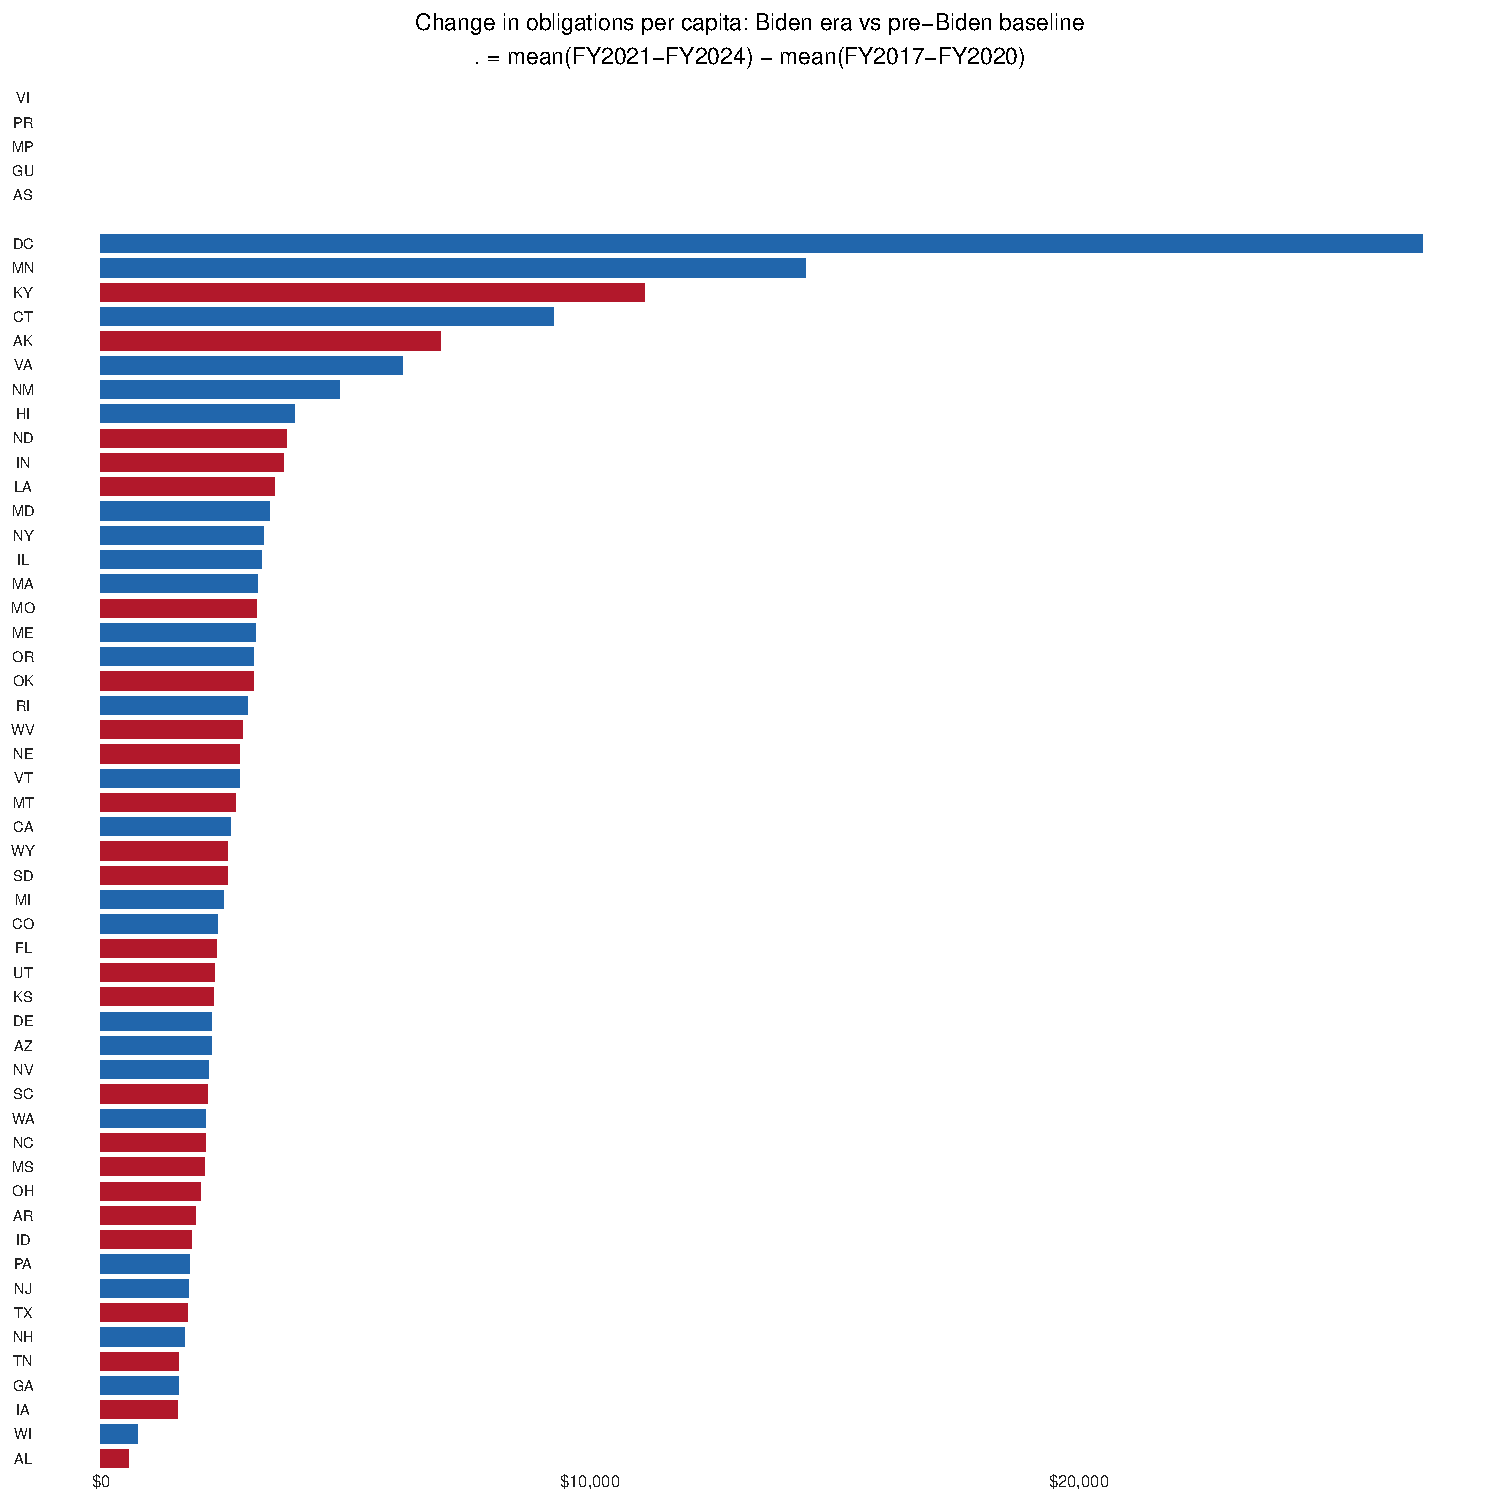
\includegraphics[keepaspectratio]{spending_elections_2020_2024_analysis_patched_files/figure-latex/delta-12-1-1.pdf}}

\subsection{Key Observations}\label{key-observations-5}

\textbf{What This Chart Shows:}

This bar chart compares average federal obligations per capita during
the Biden era (FY2021--FY2024) against the pre-Biden baseline
(FY2017--FY2020). Bars extending right indicate increased spending; bars
extending left indicate decreased spending. Colors represent which
candidate won each state in 2020 (blue = Biden, red = Trump).

\subsubsection{Spending Growth
Patterns:}\label{spending-growth-patterns}

\begin{enumerate}
\def\labelenumi{\arabic{enumi}.}
\item
  \textbf{All States Show Increases vs Pre-Biden Baseline:} Every state
  (and DC) has a \textbf{positive} per-capita change. The smallest
  increase is roughly \textbf{+\$569} (AL), while the largest is about
  \textbf{+\$27,032} (DC).
\item
  \textbf{Largest Increases Concentrated in a Few States:} The biggest
  per-capita gains are in \textbf{DC (+\$27.0k)}, \textbf{MN
  (+\$14.4k)}, \textbf{KY (+\$11.1k)}, \textbf{CT (+\$9.2k)}, and
  \textbf{AK (+\$7.0k)}. Small-population jurisdictions amplify
  per-capita effects, which helps explain DC's extreme value.
\item
  \textbf{Smallest Increases Cluster Near the Baseline:} The lowest
  increases are in \textbf{AL (+\$569)}, \textbf{WI (+\$751)},
  \textbf{IA (+\$1,572)}, \textbf{GA (+\$1,594)}, and \textbf{TN
  (+\$1,595)}, indicating relatively flat change compared to other
  states.
\end{enumerate}

\subsubsection{Political Alignment
Patterns:}\label{political-alignment-patterns}

\begin{enumerate}
\def\labelenumi{\arabic{enumi}.}
\item
  \textbf{Balanced Partisan Mix Among Increases:} The distribution of
  gains is split almost evenly: \textbf{26 Biden-won states} and
  \textbf{25 Trump-won states} show increases, indicating no simple
  partisan allocation pattern at the state level.
\item
  \textbf{Extremes Are Not Exclusively Partisan:} Large increases appear
  in both Biden-won (DC, MN, CT) and Trump-won (KY, AK) states,
  reinforcing that sectoral and programmatic factors likely dominate
  over electoral alignment.
\end{enumerate}

\subsubsection{Sectoral and Policy
Implications:}\label{sectoral-and-policy-implications}

\begin{enumerate}
\def\labelenumi{\arabic{enumi}.}
\tightlist
\item
  \textbf{Policy Over Politics:} The broad, across-the-board increases
  suggest that national policy shifts (pandemic recovery,
  infrastructure, and program growth) outweighed state-level partisan
  targeting. The scale of changes appears driven by:
\end{enumerate}

\begin{itemize}
\tightlist
\item
  Sectoral policy priorities (energy transition, infrastructure
  modernization)
\item
  Economic conditions and programmatic needs
\item
  Administrative policy shifts (pandemic program wind-downs, new
  infrastructure initiatives)
\item
  Rather than electoral reward/punishment strategies
\end{itemize}

\begin{enumerate}
\def\labelenumi{\arabic{enumi}.}
\setcounter{enumi}{2}
\tightlist
\item
  \textbf{Program Composition Matters:} Understanding which specific
  programs changed (defense spending, Medicare/Medicaid, infrastructure
  grants, energy subsidies, agricultural support) would be essential to
  fully explain these patterns.
\end{enumerate}

\subsubsection{Analytical Significance:}\label{analytical-significance}

\begin{enumerate}
\def\labelenumi{\arabic{enumi}.}
\item
  \textbf{Challenges Simple Narratives:} This chart provides evidence
  against claims that the Biden administration systematically
  ``rewarded'' states that voted Democratic in 2020: the data show no
  clear partisan pattern.
\item
  \textbf{Complex Causality:} The wide variation across states with
  different political alignments suggests federal spending patterns
  result from complex interactions of policy priorities, economic needs,
  programmatic structures, and institutional factors: not simple
  political calculations.
\item
  \textbf{Observational Analysis:} These findings represent observed
  correlations between spending changes and political characteristics.
  Causation cannot be inferred: we cannot determine whether political
  factors influenced spending, whether spending influenced politics, or
  whether both were driven by other factors.
\end{enumerate}

\section{Notes}\label{notes}

\begin{itemize}
\tightlist
\item
  Results should be interpreted as correlational.
\item
  Spending data are total federal obligations.
\item
  Further robustness checks (e.g., grants-only or agency-specific
  spending) are encouraged.
\end{itemize}

\section{Data Sources and Processing}\label{data-sources-and-processing}

This page lists local data files used in the analysis, their original
sources, and a brief summary of how each was processed.

\textbf{Summary Answer}

Spending increases in the Biden era are broad-based across states, but
the scatter plots show only moderate positive associations with 2024
presidential and House margins. The relationship is real but not
deterministic: states with similar spending changes often voted
differently, and outliers remain. In short, spending shifts alone do not
explain 2024 election outcomes, though they move in the same direction
on average.

\textbf{USAspending (federal obligations by state, FY2017--FY2024)}\\
Local file: Not stored locally (pulled live via API during analysis)\\
Source:
\url{https://api.usaspending.gov/api/v2/search/spending_by_geography/}\\
Processing: API responses are normalized to state abbreviations, then
combined with Census population to compute per-capita obligations and
multi-year averages.

\textbf{Census population estimates (2010s series)}\\
Local file: \url{NST-EST2019-ALLDATA.csv}\\
Source:
\url{https://www2.census.gov/programs-surveys/popest/datasets/2010-2019/national/totals/nst-est2019-alldata.csv}\\
Processing: Filtered to SUMLEV 40 (states + DC), then reshaped to long
format for 2017--2019 and mapped to state abbreviations.

\textbf{Census population estimates (2020s series)}\\
Local file: \url{NST-EST2024-ALLDATA.csv}\\
Source:
\url{https://www2.census.gov/programs-surveys/popest/datasets/2020-2024/state/totals/NST-EST2024-ALLDATA.csv}\\
Processing: Filtered to SUMLEV 40 (states + DC), then reshaped to long
format for 2020--2024 and mapped to state abbreviations. Combined with
2010s series to build \texttt{population\_by\_state\_fy.csv}.

\textbf{Combined population by state and fiscal year}\\
Local file: \url{population_by_state_fy.csv}\\
Source: Derived from the two Census files above\\
Processing: Union of 2017--2024 state populations with standardized
\texttt{state}, \texttt{fiscal\_year}, and \texttt{pop} fields used for
per-capita metrics.

\textbf{2024 presidential results (state level)}\\
Local file: \url{2024-electoral-states.csv}\\
Source:
\url{https://michaelminn.net/tutorials/data/2024-electoral-states.csv}\\
Processing: Cleaned column names and converted to a Democratic margin:
(Dem votes − GOP votes) / (Dem + GOP).

\textbf{2024 House results (district level)}\\
Local file: \url{2024-electoral-districts.csv}\\
Source:
\url{https://michaelminn.net/tutorials/data/2024-electoral-districts.csv}\\
Processing: Aggregated by state to compute a statewide House margin
using total Dem and GOP votes.

\textbf{2020 presidential results (for 2020 winner coloring)}\\
Local file: \url{president_2020.csv}\\
Source: User-provided (original source not embedded in the file)\\
Processing: Filtered to 2020 and the two major candidates, then assigned
a state winner based on total votes per candidate.

\textbf{IIJA funding snapshot (March 2023)}\\
Local file:
\href{IIJA\%20FUNDING\%20AS\%20OF\%20MARCH\%202023.xlsx}{IIJA FUNDING AS
OF MARCH 2023.xlsx}\\
Source: User-provided (snapshot file)\\
Processing: Loaded from Excel, mapped to state abbreviations, and
converted to per-capita values using 2023 population.

\end{document}
